%%%%%%%%%%%%%%%%%%%%%%%%%%%%%%%%%%%%%%%%%
% The Legrand Orange Book
% LaTeX Template
% Version 2.4 (26/09/2018)
%
% This template was downloaded from:
% http://www.LaTeXTemplates.com
%
% Original author:
% Mathias Legrand (legrand.mathias@gmail.com) with modifications by:
% Vel (vel@latextemplates.com)
%
% License:
% CC BY-NC-SA 3.0 (http://creativecommons.org/licenses/by-nc-sa/3.0/)
%
% Compiling this template:
% This template uses biber for its bibliography and makeindex for its index.
% When you first open the template, compile it from the command line with the 
% commands below to make sure your LaTeX distribution is configured correctly:
%
% 1) pdflatex main
% 2) makeindex main.idx -s StyleInd.ist
% 3) biber main
% 4) pdflatex main x 2
%
% After this, when you wish to update the bibliography/index use the appropriate
% command above and make sure to compile with pdflatex several times 
% afterwards to propagate your changes to the document.
%
% This template also uses a number of packages which may need to be
% updated to the newest versions for the template to compile. It is strongly
% recommended you update your LaTeX distribution if you have any
% compilation errors.
%
% Important note:
% Chapter heading images should have a 2:1 width:height ratio,
% e.g. 920px width and 460px height.
%
%%%%%%%%%%%%%%%%%%%%%%%%%%%%%%%%%%%%%%%%%

%----------------------------------------------------------------------------------------
%	CONTENTS COMPILATION CONTROL
%----------------------------------------------------------------------------------------

% \newcommand*{\printdemo}{}
\newcommand*{\printvocabulary}{}

%----------------------------------------------------------------------------------------
%	PACKAGES AND OTHER DOCUMENT CONFIGURATIONS
%----------------------------------------------------------------------------------------

\documentclass[11pt,fleqn]{book} % Default font size and left-justified equations

%%%%%%%%%%%%%%%%%%%%%%%%%%%%%%%%%%%%%%%%%
% The Legrand Orange Book
% Structural Definitions File
% Version 2.1 (26/09/2018)
%
% Original author:
% Mathias Legrand (legrand.mathias@gmail.com) with modifications by:
% Vel (vel@latextemplates.com)
% 
% This file was downloaded from:
% http://www.LaTeXTemplates.com
%
% License:
% CC BY-NC-SA 3.0 (http://creativecommons.org/licenses/by-nc-sa/3.0/)
%
%%%%%%%%%%%%%%%%%%%%%%%%%%%%%%%%%%%%%%%%%

%----------------------------------------------------------------------------------------
%	VARIOUS REQUIRED PACKAGES AND CONFIGURATIONS
%----------------------------------------------------------------------------------------

\usepackage{graphicx} % Required for including pictures
\graphicspath{{Pictures/}} % Specifies the directory where pictures are stored

\usepackage{lipsum} % Inserts dummy text

\usepackage{tikz} % Required for drawing custom shapes

\usepackage[english]{babel} % English language/hyphenation

\usepackage{enumitem} % Customize lists
\setlist{nolistsep} % Reduce spacing between bullet points and numbered lists

\usepackage{booktabs} % Required for nicer horizontal rules in tables

\usepackage{xcolor} % Required for specifying colors by name
% \definecolor{ocre}{RGB}{243,102,25} % Define the orange color used for highlighting throughout the book
\definecolor{ocre}{RGB}{76, 50, 168}
\definecolor{coral}{RGB}{184, 84, 80}

\usepackage{calc}

%----------------------------------------------------------------------------------------
%	My Custom Packages
%----------------------------------------------------------------------------------------
% unused packages
% \usepackage{thmtools}
% \usepackage{xpatch}
% \xpatchcmd{\listoftheorems}{\@fileswfalse}{}{\typeout{yes}}{\typeout{no}}

%	IPA
% \usepackage{unitipa}


\usepackage{algorithm2e}
\usepackage{tabularx} % adjustable width tables
\usepackage{svg}

% for sub figure
\usepackage{caption}
\usepackage{subcaption}

%----------------------------------------------------------------------------------------
%	MARGINS
%----------------------------------------------------------------------------------------

\usepackage{geometry} % Required for adjusting page dimensions and margins

\geometry{
	paper=a4paper, % Paper size, change to letterpaper for US letter size
	top=3cm, % Top margin
	bottom=3cm, % Bottom margin
	left=3cm, % Left margin
	right=3cm, % Right margin
	headheight=14pt, % Header height
	footskip=1.4cm, % Space from the bottom margin to the baseline of the footer
	headsep=10pt, % Space from the top margin to the baseline of the header
	%showframe, % Uncomment to show how the type block is set on the page
}

%----------------------------------------------------------------------------------------
%	FONTS
%----------------------------------------------------------------------------------------


% \usepackage{avant} % Use the Avantgarde font for headings
%\usepackage{times} % Use the Times font for headings
% \usepackage{mathptmx} % Use the Adobe Times Roman as the default text font together with math symbols from the Sym­bol, Chancery and Com­puter Modern fonts

\usepackage{microtype} % Slightly tweak font spacing for aesthetics
%\usepackage[utf8]{inputenc} % Required for including letters with accents
\usepackage[T1]{fontenc} % Use 8-bit encoding that has 256 glyphs

% support CJK characters
\usepackage{xeCJK}

\setmainfont[BoldFont=NotoSerif-Bold.ttf, ItalicFont=NotoSerif-Italic.ttf]{NotoSerif-Regular.ttf}
% \setmainfont[ItalicFont=NotoSerif-Italic.ttf]{RobotoSlab-VariableFont_wght.ttf}
% \setsansfont{Fira Sans}
% \setsansfont{Open Sans}
% \setsansfont[BoldFont=SegUIVar.ttf, ItalicFont=SegUIVar.ttf]{SegUIVar.ttf}

\setmonofont{Cascadia Code}
\setCJKmainfont[BoldFont=PingFang Heavy.ttf,ItalicFont=FZKTK.TTF]{FZPingXYSJW.TTF}
\setCJKsansfont[BoldFont=PingFang Heavy.ttf,ItalicFont=PingFang Heavy.ttf]{PingFang Heavy.ttf}
\setCJKmonofont[BoldFont=PingFang Heavy.ttf,ItalicFont=PingFang Heavy.ttf]{FZFSK.TTF}
\xeCJKsetup{CJKmath = true}

% support chemical equation arrows
\usepackage[version=4]{mhchem}
% \renewcommand{\rmdefault}{noto}
% \renewcommand{\familydefault}{\sfdefault}

%----------------------------------------------------------------------------------------
%	BIBLIOGRAPHY AND INDEX
%----------------------------------------------------------------------------------------

\usepackage[style=numeric,citestyle=numeric,sorting=nyt,sortcites=true,autopunct=true,babel=hyphen,hyperref=true,abbreviate=false,backref=true,backend=biber]{biblatex}
\addbibresource{E:/OneDrive/Library/library.bib}
% \addbibresource{bibliography.bib} % BibTeX bibliography file
\defbibheading{bibempty}{}

\usepackage{calc} % For simpler calculation - used for spacing the index letter headings correctly
\usepackage{makeidx} % Required to make an index
\makeindex % Tells LaTeX to create the files required for indexing

%----------------------------------------------------------------------------------------
%	MAIN TABLE OF CONTENTS
%----------------------------------------------------------------------------------------

\usepackage{titletoc} % Required for manipulating the table of contents

\contentsmargin{0cm} % Removes the default margin

% Part text styling (this is mostly taken care of in the PART HEADINGS section of this file)
\titlecontents{part}
	[0cm] % Left indentation
	{\addvspace{20pt}\bfseries} % Spacing and font options for parts
	{}
	{}
	{}

% Chapter text styling
\titlecontents{chapter}
	[1.25cm] % Left indentation
	{\addvspace{12pt}\large\sffamily\bfseries} % Spacing and font options for chapters
	{\color{ocre!60}\contentslabel[\Large\thecontentslabel]{1.25cm}\color{ocre}} % Formatting of numbered sections of this type
	{\color{ocre}} % Formatting of numberless sections of this type
	{\color{ocre!60}\normalsize\;\titlerule*[.5pc]{.}\;\thecontentspage} % Formatting of the filler to the right of the heading and the page number

% Section text styling
\titlecontents{section}
	[1.25cm] % Left indentation
	{\addvspace{3pt}\sffamily\bfseries} % Spacing and font options for sections
	{\contentslabel[\thecontentslabel]{1.25cm}} % Formatting of numbered sections of this type
	{} % Formatting of numberless sections of this type
	{\hfill\color{black}\thecontentspage} % Formatting of the filler to the right of the heading and the page number

% Subsection text styling
\titlecontents{subsection}
	[1.25cm] % Left indentation
	{\addvspace{1pt}\sffamily\small} % Spacing and font options for subsections
	{\contentslabel[\thecontentslabel]{1.25cm}} % Formatting of numbered sections of this type
	{} % Formatting of numberless sections of this type
	{\ \titlerule*[.5pc]{.}\;\thecontentspage} % Formatting of the filler to the right of the heading and the page number

% Figure text styling
\titlecontents{figure}
	[1.25cm] % Left indentation
	{\addvspace{1pt}\sffamily\small} % Spacing and font options for figures
	{\thecontentslabel\hspace*{1em}} % Formatting of numbered sections of this type
	{} % Formatting of numberless sections of this type
	{\ \titlerule*[.5pc]{.}\;\thecontentspage} % Formatting of the filler to the right of the heading and the page number

% Table text styling
\titlecontents{table}
	[1.25cm] % Left indentation
	{\addvspace{1pt}\sffamily\small} % Spacing and font options for tables
	{\thecontentslabel\hspace*{1em}} % Formatting of numbered sections of this type
	{} % Formatting of numberless sections of this type
	{\ \titlerule*[.5pc]{.}\;\thecontentspage} % Formatting of the filler to the right of the heading and the page number

%----------------------------------------------------------------------------------------
%	MINI TABLE OF CONTENTS IN PART HEADS
%----------------------------------------------------------------------------------------

% Chapter text styling
\titlecontents{lchapter}
	[0em] % Left indentation
	{\addvspace{15pt}\large\sffamily\bfseries} % Spacing and font options for chapters
	{\color{ocre}\contentslabel[\Large\thecontentslabel]{1.25cm}\color{ocre}} % Chapter number
	{}  
	{\color{ocre}\normalsize\sffamily\bfseries\;\titlerule*[.5pc]{.}\;\thecontentspage} % Page number

% Section text styling
\titlecontents{lsection}
	[0em] % Left indentation
	{\sffamily\small} % Spacing and font options for sections
	{\contentslabel[\thecontentslabel]{1.25cm}} % Section number
	{}
	{}

% Subsection text styling (note these aren't shown by default, display them by searchings this file for tocdepth and reading the commented text)
\titlecontents{lsubsection}
	[.5em] % Left indentation
	{\sffamily\footnotesize} % Spacing and font options for subsections
	{\contentslabel[\thecontentslabel]{1.25cm}}
	{}
	{}

%----------------------------------------------------------------------------------------
%	HEADERS AND FOOTERS
%----------------------------------------------------------------------------------------

\usepackage{fancyhdr} % Required for header and footer configuration

\pagestyle{fancy} % Enable the custom headers and footers

\renewcommand{\chaptermark}[1]{\markboth{\sffamily\normalsize\bfseries\chaptername\ \thechapter.\ #1}{}} % Styling for the current chapter in the header
\renewcommand{\sectionmark}[1]{\markright{\sffamily\normalsize\thesection\hspace{5pt}#1}{}} % Styling for the current section in the header

\fancyhf{} % Clear default headers and footers
\fancyhead[LE,RO]{\sffamily\normalsize\thepage} % Styling for the page number in the header
\fancyhead[LO]{\rightmark} % Print the nearest section name on the left side of odd pages
\fancyhead[RE]{\leftmark} % Print the current chapter name on the right side of even pages
%\fancyfoot[C]{\thepage} % Uncomment to include a footer

\renewcommand{\headrulewidth}{0.5pt} % Thickness of the rule under the header

\fancypagestyle{plain}{% Style for when a plain pagestyle is specified
	\fancyhead{}\renewcommand{\headrulewidth}{0pt}%
}

% Removes the header from odd empty pages at the end of chapters
\makeatletter
\renewcommand{\cleardoublepage}{
\clearpage\ifodd\c@page\else
\hbox{}
\vspace*{\fill}
\thispagestyle{empty}
\newpage
\fi}

%----------------------------------------------------------------------------------------
%	THEOREM STYLES
%----------------------------------------------------------------------------------------

\usepackage{amsmath,amsfonts,amssymb,amsthm} % For math equations, theorems, symbols, etc

\newcommand{\intoo}[2]{\mathopen{]}#1\,;#2\mathclose{[}}
\newcommand{\ud}{\mathop{\mathrm{{}d}}\mathopen{}}
\newcommand{\intff}[2]{\mathopen{[}#1\,;#2\mathclose{]}}
\renewcommand{\qedsymbol}{$\blacksquare$}
\newtheorem{notation}{Notation}[chapter]

% Boxed/framed environments
\newtheoremstyle{ocrenumbox}% Theorem style name
{0pt}% Space above
{0pt}% Space below
{\normalfont}% Body font
{}% Indent amount
{\small\bf\sffamily\color{ocre}}% Theorem head font
{\;}% Punctuation after theorem head
{0.25em}% Space after theorem head
{\small\sffamily\color{ocre}\thmname{#1}\nobreakspace\thmnumber{\@ifnotempty{#1}{}\@upn{#2}}% Theorem text (e.g. Theorem 2.1)
\thmnote{\nobreakspace\the\thm@notefont\sffamily\bfseries\color{black}---\nobreakspace#3.}} % Optional theorem note

\newtheoremstyle{blacknumex}% Theorem style name
{5pt}% Space above
{5pt}% Space below
{\normalfont}% Body font
{} % Indent amount
{\small\bf\sffamily}% Theorem head font
{\;}% Punctuation after theorem head
{0.25em}% Space after theorem head
{\small\sffamily{\tiny\ensuremath{\blacksquare}}\nobreakspace\thmname{#1}\nobreakspace\thmnumber{\@ifnotempty{#1}{}\@upn{#2}}% Theorem text (e.g. Theorem 2.1)
\thmnote{\nobreakspace\the\thm@notefont\sffamily\bfseries---\nobreakspace#3.}}% Optional theorem note

\newtheoremstyle{blacknumbox} % Theorem style name
{0pt}% Space above
{0pt}% Space below
{\normalfont}% Body font
{}% Indent amount
{\small\bf\sffamily}% Theorem head font
{\;}% Punctuation after theorem head
{0.25em}% Space after theorem head
{\small\sffamily\thmname{#1}\nobreakspace\thmnumber{\@ifnotempty{#1}{}\@upn{#2}}% Theorem text (e.g. Theorem 2.1)
\thmnote{\nobreakspace\the\thm@notefont\sffamily\bfseries---\nobreakspace#3.}}% Optional theorem note

\newtheoremstyle{blacknumboxSpecial} % Theorem style name
{0pt}% Space above
{0pt}% Space below
{\normalfont}% Body font
{}% Indent amount
{\small\bf\sffamily}% Theorem head font
{\;}% Punctuation after theorem head
{0.25em}% Space after theorem head
{\small\sffamily\thmname{#1}\nobreakspace\thmnumber{\@ifnotempty{#1}{}\@upn{#2}}% Theorem text (e.g. Theorem 2.1)
\thmnote{\nobreakspace\the\thm@notefont\sffamily\bfseries---\nobreakspace#3.}}% Optional theorem note


% Non-boxed/non-framed environments
\newtheoremstyle{ocrenum}% Theorem style name
{5pt}% Space above
{5pt}% Space below
{\normalfont}% Body font
{}% Indent amount
{\small\bf\sffamily\color{ocre}}% Theorem head font
{\;}% Punctuation after theorem head
{0.25em}% Space after theorem head
{\small\sffamily\color{ocre}\thmname{#1}\nobreakspace\thmnumber{\@ifnotempty{#1}{}\@upn{#2}}% Theorem text (e.g. Theorem 2.1)
\thmnote{\nobreakspace\the\thm@notefont\sffamily\bfseries\color{black}---\nobreakspace#3.}} % Optional theorem note
\makeatother

% Defines the theorem text style for each type of theorem to one of the three styles above
\newcounter{dummy} 
\numberwithin{dummy}{section}
\theoremstyle{ocrenumbox}
\newtheorem{theoremeT}[dummy]{Theorem}
\newtheorem{problem}{Problem}[chapter]
\newtheorem{exerciseT}{Exercise}[chapter]
\theoremstyle{blacknumex}
\newtheorem{exampleT}{Example}[chapter]
\theoremstyle{blacknumboxSpecial} 
\newtheorem{vocabulary}{Vocabulary}[chapter]
\theoremstyle{blacknumbox}
\newtheorem{definitionT}{Definition}[section]
\newtheorem{corollaryT}[dummy]{Corollary}
\theoremstyle{ocrenum}
\newtheorem{proposition}[dummy]{Proposition}

% use ``word'' environment to wrap vocabulary and add index
% \newenvironment{DefWord}[1]{\begin{vocabulary}[#1] \index{#1}}{ \end{vocabulary}}

% define new environment: RefWord and DefWord for vocabulary.
\usepackage{xparse}
\NewDocumentEnvironment{RefWord}{ m o}{
	% Start Code
	\IfNoValueTF{#2}{
		% if optional parameter is null
		\begin{vocabulary}[#1]
			\index{#1}
			% See \textbf{#1} (Vocabulary \ref{#1}).
			\hyperref[#1]{  $\rightarrow$ V \ref{#1}}.
		}{
		\begin{vocabulary}[#1]
			\index{#2}
			\hyperref[#2]{$\rightarrow$ \texttt{#2} (V \ref{#2})}.
			
	}
}{	% End Code
		\end{vocabulary}
}
\NewDocumentEnvironment{DefWord}{mo}{
	% Start Code
	\IfNoValueTF{#2}{
		\begin{vocabulary}[#1]
			\label{#1}
			\index{#1}
		}{
		\begin{vocabulary}[#1]
			\label{#2}
			\index{#2}
	}
}{% End Code
		\end{vocabulary}
}
\newcommand{\term}[1]{\textit{#1}\index{#1}}

%----------------------------------------------------------------------------------------
%	DEFINITION OF COLORED BOXES
%----------------------------------------------------------------------------------------

\RequirePackage[framemethod=default]{mdframed} % Required for creating the theorem, definition, exercise and corollary boxes

% Theorem box
\newmdenv[skipabove=7pt,
skipbelow=7pt,
backgroundcolor=black!5,
linecolor=ocre,
innerleftmargin=5pt,
innerrightmargin=5pt,
innertopmargin=5pt,
leftmargin=0cm,
rightmargin=0cm,
innerbottommargin=5pt]{tBox}

% Exercise box	  
\newmdenv[skipabove=7pt,
skipbelow=7pt,
rightline=false,
leftline=true,
topline=false,
bottomline=false,
backgroundcolor=ocre!10,
linecolor=ocre,
innerleftmargin=5pt,
innerrightmargin=5pt,
innertopmargin=5pt,
innerbottommargin=5pt,
leftmargin=0cm,
rightmargin=0cm,
linewidth=4pt]{eBox}	

% Definition box
\newmdenv[skipabove=7pt,
skipbelow=7pt,
rightline=false,
leftline=true,
topline=false,
bottomline=false,
linecolor=ocre,
innerleftmargin=5pt,
innerrightmargin=5pt,
innertopmargin=0pt,
leftmargin=0cm,
rightmargin=0cm,
linewidth=4pt,
innerbottommargin=0pt]{dBox}	

% Corollary box
\newmdenv[skipabove=7pt,
skipbelow=7pt,
rightline=false,
leftline=true,
topline=false,
bottomline=false,
linecolor=gray,
backgroundcolor=black!5,
innerleftmargin=5pt,
innerrightmargin=5pt,
innertopmargin=5pt,
leftmargin=0cm,
rightmargin=0cm,
linewidth=4pt,
innerbottommargin=5pt]{cBox}

% Creates an environment for each type of theorem and assigns it a theorem text style from the "Theorem Styles" section above and a colored box from above
\newenvironment{theorem}{\begin{tBox}\begin{theoremeT}}{\end{theoremeT}\end{tBox}}
\newenvironment{exercise}{\begin{eBox}\begin{exerciseT}}{\hfill{\color{ocre}\tiny\ensuremath{\blacksquare}}\end{exerciseT}\end{eBox}}				  
\newenvironment{definition}{\begin{dBox}\begin{definitionT}}{\end{definitionT}\end{dBox}}	
\newenvironment{example}{\begin{exampleT}}{\hfill{\tiny\ensuremath{\blacksquare}}\end{exampleT}}		
\newenvironment{corollary}{\begin{cBox}\begin{corollaryT}}{\end{corollaryT}\end{cBox}}	
% \newenvironment{algorithmNew}[1]{\begin{cBox}\begin{algorithm} \caption{#1} }{\end{algorithm}\end{cBox}}


%----------------------------------------------------------------------------------------
%	REMARK ENVIRONMENT
%----------------------------------------------------------------------------------------

\newenvironment{remark}{\par\vspace{0.125pt}\small % Vertical white space above the remark and smaller font size
\begin{list}{}{
\leftmargin=35pt % Indentation on the left
\rightmargin=25pt}\item\ignorespaces % Indentation on the right

%\makebox[-2.5pt]{
	
\begin{tikzpicture}[overlay]
\node[draw=coral!60,line width=1pt,circle,fill=coral!25,font=\sffamily\bfseries,inner sep=2pt,outer sep=0pt] at (-15pt,0pt){\textcolor{coral}{!}};\end{tikzpicture}

%} % Orange ! in a circle

% Candidate 1 (use svg directly)
%\makebox[-1pt]{
	%\begin{figure}[htbp]
		%
\includegraphics[scale=1,bb=0 0 30 30]{remarksymbol.svg}
		%
\includegraphics{remarksymbol.svg}
		%
\includegraphics[scale=0.25]{remarkSymbol.png}
	%\end{figure}
%}


\advance\baselineskip -0.5pt}{\end{list}\vskip0.125pt} % Tighter line spacing and white space after remark

% Candidate 2 (use png)
%\newenvironment{remark}{\begin{figure}[htbp]
%	\centering
%	
\includegraphics{remarkSymbol.png}
%\end{figure}}{}


%----------------------------------------------------------------------------------------
%	SECTION NUMBERING IN THE MARGIN
%----------------------------------------------------------------------------------------

\makeatletter
\renewcommand{\@seccntformat}[1]{\llap{\textcolor{ocre}{\csname the#1\endcsname}\hspace{1em}}}                    
\renewcommand{\section}{\@startsection{section}{1}{\z@}
{-4ex \@plus -1ex \@minus -.4ex}
{1ex \@plus.2ex }
{\normalfont\large\sffamily\bfseries}}
\renewcommand{\subsection}{\@startsection {subsection}{2}{\z@}
{-3ex \@plus -0.1ex \@minus -.4ex}
{0.5ex \@plus.2ex }
{\normalfont\sffamily\bfseries}}
\renewcommand{\subsubsection}{\@startsection {subsubsection}{3}{\z@}
{-2ex \@plus -0.1ex \@minus -.2ex}
{.2ex \@plus.2ex }
{\normalfont\small\sffamily\bfseries}}                        
\renewcommand\paragraph{\@startsection{paragraph}{4}{\z@}
{-2ex \@plus-.2ex \@minus .2ex}
{.1ex}
{\normalfont\small\sffamily\bfseries}}

%----------------------------------------------------------------------------------------
%	PART HEADINGS
%----------------------------------------------------------------------------------------

% Numbered part in the table of contents
\newcommand{\@mypartnumtocformat}[2]{%
	\setlength\fboxsep{0pt}%
	\noindent\colorbox{ocre!20}{\strut\parbox[c][.7cm]{\ecart}{\color{ocre!70}\Large\sffamily\bfseries\centering#1}}\hskip\esp\colorbox{ocre!40}{\strut\parbox[c][.7cm]{\linewidth-\ecart-\esp}{\Large\sffamily\centering#2}}%
}

% Unnumbered part in the table of contents
\newcommand{\@myparttocformat}[1]{%
	\setlength\fboxsep{0pt}%
	\noindent\colorbox{ocre!40}{\strut\parbox[c][.7cm]{\linewidth}{\Large\sffamily\centering#1}}%
}

\newlength\esp
\setlength\esp{4pt}
\newlength\ecart
\setlength\ecart{1.2cm-\esp}
\newcommand{\thepartimage}{}%
\newcommand{\partimage}[1]{\renewcommand{\thepartimage}{#1}}%
\def\@part[#1]#2{%
\ifnum \c@secnumdepth >-2\relax%
\refstepcounter{part}%
\addcontentsline{toc}{part}{\texorpdfstring{\protect\@mypartnumtocformat{\thepart}{#1}}{\partname~\thepart\ ---\ #1}}
\else%
\addcontentsline{toc}{part}{\texorpdfstring{\protect\@myparttocformat{#1}}{#1}}%
\fi%
\startcontents%
\markboth{}{}%
{\thispagestyle{empty}%
\begin{tikzpicture}[remember picture,overlay]%
\node at (current page.north west){\begin{tikzpicture}[remember picture,overlay]%	
\fill[ocre!20](0cm,0cm) rectangle (\paperwidth,-\paperheight);
\node[anchor=north] at (4cm,-3.25cm){\color{ocre!40}\fontsize{220}{100}\sffamily\bfseries\thepart}; 
\node[anchor=south east] at (\paperwidth-1cm,-\paperheight+1cm){\parbox[t][][t]{8.5cm}{
\printcontents{l}{0}{\setcounter{tocdepth}{1}}% The depth to which the Part mini table of contents displays headings; 0 for chapters only, 1 for chapters and sections and 2 for chapters, sections and subsections
}};
\node[anchor=north east] at (\paperwidth-1.5cm,-3.25cm){\parbox[t][][t]{15cm}{\strut\raggedleft\color{white}\fontsize{30}{30}\sffamily\bfseries#2}};
\end{tikzpicture}};
\end{tikzpicture}}%
\@endpart}
\def\@spart#1{%
\startcontents%
\phantomsection
{\thispagestyle{empty}%
\begin{tikzpicture}[remember picture,overlay]%
\node at (current page.north west){\begin{tikzpicture}[remember picture,overlay]%	
\fill[ocre!20](0cm,0cm) rectangle (\paperwidth,-\paperheight);
\node[anchor=north east] at (\paperwidth-1.5cm,-3.25cm){\parbox[t][][t]{15cm}{\strut\raggedleft\color{white}\fontsize{30}{30}\sffamily\bfseries#1}};
\end{tikzpicture}};
\end{tikzpicture}}
\addcontentsline{toc}{part}{\texorpdfstring{%
\setlength\fboxsep{0pt}%
\noindent\protect\colorbox{ocre!40}{\strut\protect\parbox[c][.7cm]{\linewidth}{\Large\sffamily\protect\centering #1\quad\mbox{}}}}{#1}}%
\@endpart}
\def\@endpart{\vfil\newpage
\if@twoside
\if@openright
\null
\thispagestyle{empty}%
\newpage
\fi
\fi
\if@tempswa
\twocolumn
\fi}

%----------------------------------------------------------------------------------------
%	CHAPTER HEADINGS
%----------------------------------------------------------------------------------------

% A switch to conditionally include a picture, implemented by Christian Hupfer
\newif\ifusechapterimage
\usechapterimagetrue
\newcommand{\thechapterimage}{}%
\newcommand{\chapterimage}[1]{\ifusechapterimage\renewcommand{\thechapterimage}{#1}\fi}%
\newcommand{\autodot}{.}
\def\@makechapterhead#1{%
{\parindent \z@ \raggedright \normalfont
\ifnum \c@secnumdepth >\m@ne
\if@mainmatter
\begin{tikzpicture}[remember picture,overlay]
\node at (current page.north west)
{\begin{tikzpicture}[remember picture,overlay]
\node[anchor=north west,inner sep=0pt] at (0,0) {\ifusechapterimage\includegraphics[width=\paperwidth]{\thechapterimage}\fi};
\draw[anchor=west] (\Gm@lmargin,-9cm) node [line width=2pt,rounded corners=15pt,draw=ocre,fill=white,fill opacity=0.5,inner sep=15pt]{\strut\makebox[22cm]{}};
\draw[anchor=west] (\Gm@lmargin+.3cm,-9cm) node {\huge\sffamily\bfseries\color{black}\thechapter\autodot~#1\strut};
\end{tikzpicture}};
\end{tikzpicture}
\else
\begin{tikzpicture}[remember picture,overlay]
\node at (current page.north west)
{\begin{tikzpicture}[remember picture,overlay]
\node[anchor=north west,inner sep=0pt] at (0,0) {\ifusechapterimage\includegraphics[width=\paperwidth]{\thechapterimage}\fi};
\draw[anchor=west] (\Gm@lmargin,-9cm) node [line width=2pt,rounded corners=15pt,draw=ocre,fill=white,fill opacity=0.5,inner sep=15pt]{\strut\makebox[22cm]{}};
\draw[anchor=west] (\Gm@lmargin+.3cm,-9cm) node {\huge\sffamily\bfseries\color{black}#1\strut};
\end{tikzpicture}};
\end{tikzpicture}
\fi\fi\par\vspace*{270\p@}}}

%-------------------------------------------

\def\@makeschapterhead#1{%
\begin{tikzpicture}[remember picture,overlay]
\node at (current page.north west)
{\begin{tikzpicture}[remember picture,overlay]
\node[anchor=north west,inner sep=0pt] at (0,0) {\ifusechapterimage\includegraphics[width=\paperwidth]{\thechapterimage}\fi};
\draw[anchor=west] (\Gm@lmargin,-9cm) node [line width=2pt,rounded corners=15pt,draw=ocre,fill=white,fill opacity=0.5,inner sep=15pt]{\strut\makebox[22cm]{}};
\draw[anchor=west] (\Gm@lmargin+.3cm,-9cm) node {\huge\sffamily\bfseries\color{black}#1\strut};
\end{tikzpicture}};
\end{tikzpicture}
\par\vspace*{270\p@}}
\makeatother

%----------------------------------------------------------------------------------------
%	LINKS
%----------------------------------------------------------------------------------------

\usepackage{hyperref}
\hypersetup{hidelinks,backref=true,pagebackref=true,hyperindex=true,colorlinks=false,breaklinks=true,urlcolor=ocre,bookmarks=true,bookmarksopen=false}

\usepackage{bookmark}
\bookmarksetup{
open,
numbered,
addtohook={%
\ifnum\bookmarkget{level}=0 % chapter
\bookmarksetup{bold}%
\fi
\ifnum\bookmarkget{level}=-1 % part
\bookmarksetup{color=ocre,bold}%
\fi
}
}

% cleveref must be loaded after amsmath
\usepackage{cleveref}

% for the long section
% \section[Hidden Markov Map Matching Through Noise and Sparseness]{\texorpdfstring{Hidden Markov Map Matching\\ Through Noise and Sparseness}{Hidden Markov Map Matching Through Noise and Sparseness}}
% the optional parameter is for TOC display, the second one is for TeX display, the third one is for PDF string % Insert the commands.tex file which contains the majority of the structure behind the template

%\hypersetup{pdftitle={Title},pdfauthor={Author}} % Uncomment and fill out to include PDF metadata for the author and title of the book

%----------------------------------------------------------------------------------------

\begin{document}

%----------------------------------------------------------------------------------------
%	TITLE PAGE
%----------------------------------------------------------------------------------------

\begingroup
\thispagestyle{empty} % Suppress headers and footers on the title page
\begin{tikzpicture}[remember picture,overlay]
\node[inner sep=0pt] (background) at (current page.center) {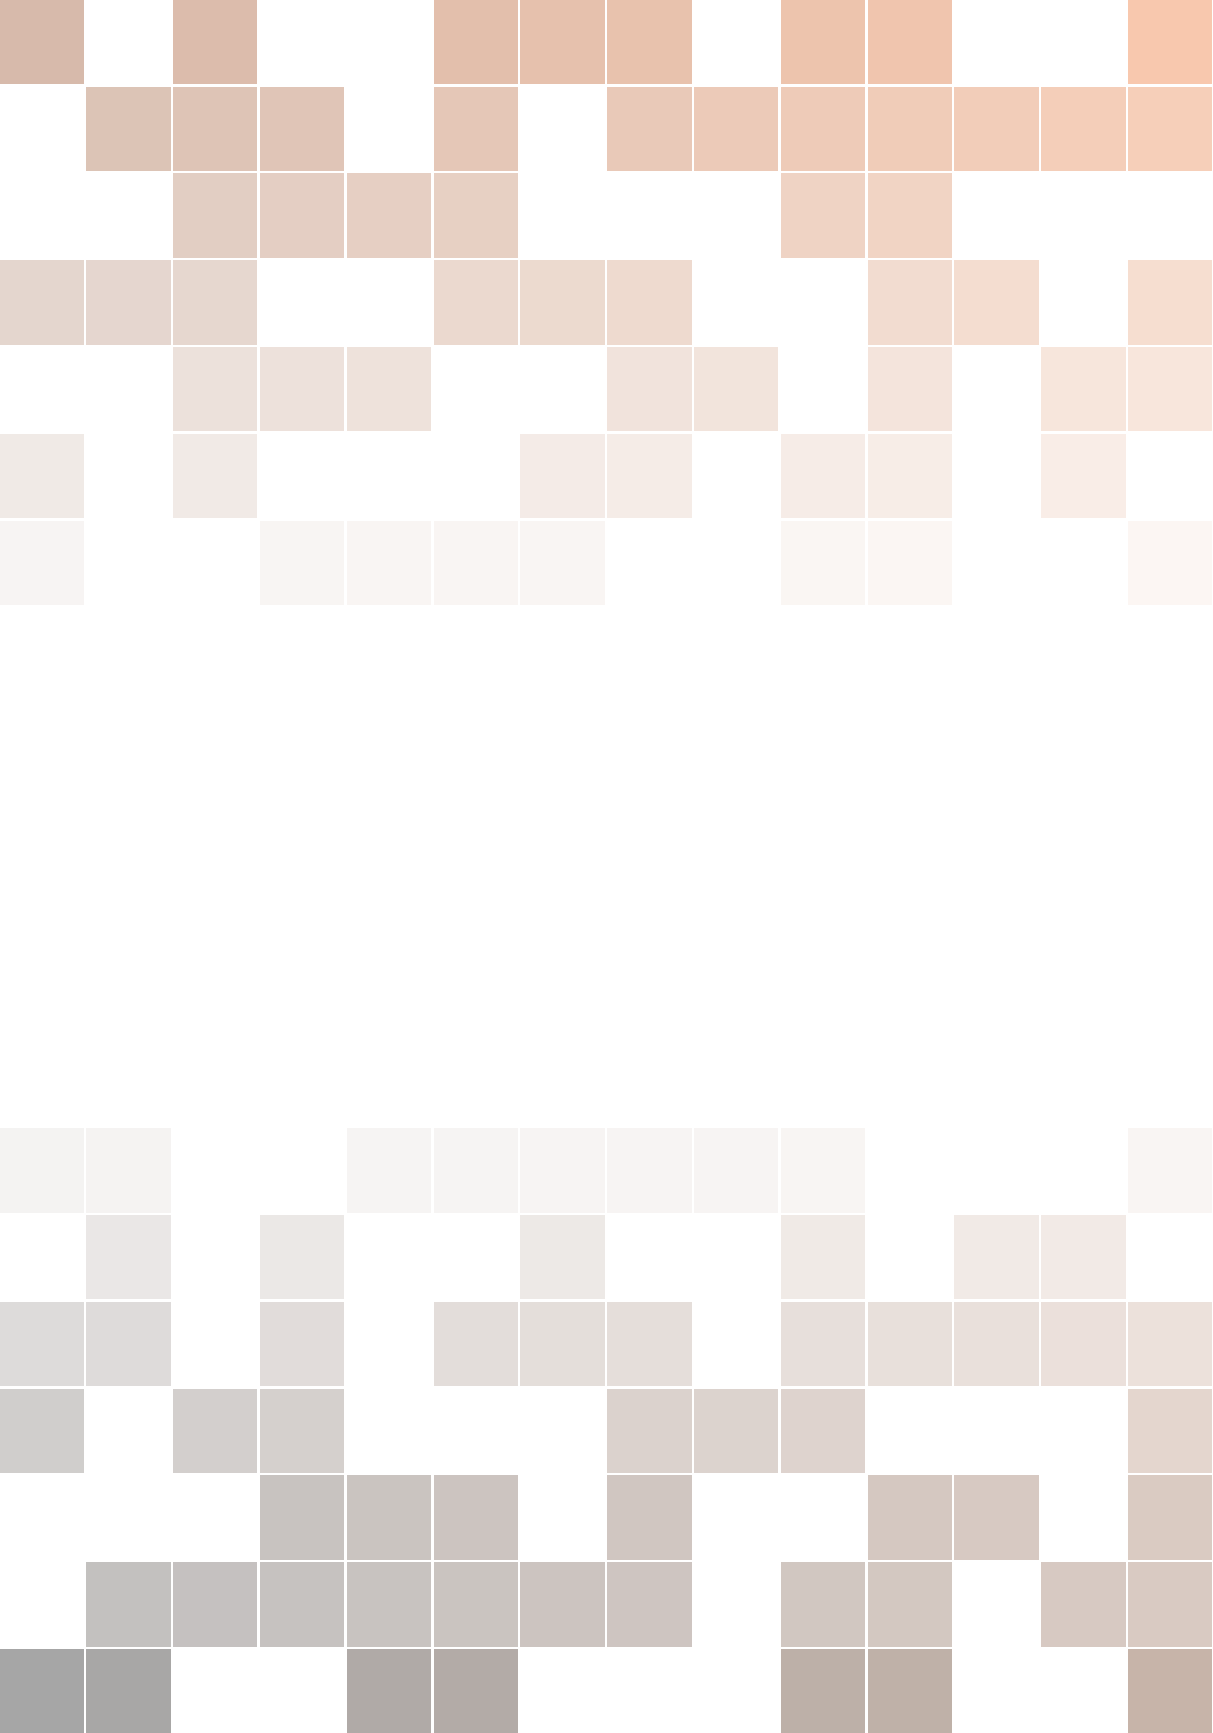
\includegraphics[width=\paperwidth]{background.pdf}};
\draw (current page.center) node [fill=ocre!30!white,fill opacity=0.6,text opacity=1,inner sep=1cm]{\Huge\centering\bfseries\sffamily\parbox[c][][t]{\paperwidth}{\centering The Search for a Title\\[15pt] % Book title
{\Large A Profound Subtitle}\\[20pt] % Subtitle
{\huge Dr. John Smith}}}; % Author name
\end{tikzpicture}
\vfill
\endgroup

%----------------------------------------------------------------------------------------
%	COPYRIGHT PAGE
%----------------------------------------------------------------------------------------

\newpage
~\vfill
\thispagestyle{empty}

\noindent Copyright \copyright\ 2019 John Smith\\ % Copyright notice

\noindent \textsc{Published by Publisher}\\ % Publisher

\noindent \textsc{book-website.com}\\ % URL

\noindent Licensed under the Creative Commons Attribution-NonCommercial 3.0 Unported License (the ``License''). You may not use this file except in compliance with the License. You may obtain a copy of the License at \url{http://creativecommons.org/licenses/by-nc/3.0}. Unless required by applicable law or agreed to in writing, software distributed under the License is distributed on an \textsc{``as is'' basis, without warranties or conditions of any kind}, either express or implied. See the License for the specific language governing permissions and limitations under the License.\\ % License information, replace this with your own license (if any)

\noindent \textit{First printing, March 2019} % Printing/edition date

%----------------------------------------------------------------------------------------
%	TABLE OF CONTENTS
%----------------------------------------------------------------------------------------

%\usechapterimagefalse % If you don't want to include a chapter image, use this to toggle images off - it can be enabled later with \usechapterimagetrue

\chapterimage{chapter_head_1.pdf} % Table of contents heading image

\pagestyle{empty} % Disable headers and footers for the following pages

\tableofcontents % Print the table of contents itself

\cleardoublepage % Forces the first chapter to start on an odd page so it's on the right side of the book

\pagestyle{fancy} % Enable headers and footers again


%----------------------------------------------------------------------------------------
%	PART 1: Vocabulary
%----------------------------------------------------------------------------------------

\part{Part One}

%----------------------------------------------------------------------------------------
%	Vocabulary (USING CONDITIONAL COMPILATION)
%----------------------------------------------------------------------------------------

\ifdefined\printvocabulary
\ifdefined\printvocabulary

\part{All Roots}
% roots
\chapter{Hearing, Seeing, Saying, Doing}

\section{vis}
\begin{wordRef}{visual, visualize}[visual]
\end{wordRef}

\begin{wordRef}{visible, visibility, invisible}[visible]
\end{wordRef}

\section{audi- (声音)}
\begin{wordRef}{audio}
\end{wordRef}

\begin{wordRef}{audience}
\end{wordRef}

\begin{wordRef}{audition}
\end{wordRef}

\section{{ag- (做,加强)}}

\begin{wordRef}{agenda}
\end{wordRef}

\begin{wordRef}{agency}
\end{wordRef}

\begin{wordRef}{agent}
\end{wordRef}

\begin{wordRef}{aggress, aggressive, aggressor}[aggress]
\end{wordRef}

\section{dict (doing)}

\begin{wordRef}{predict, prediction, predictable, unpredictable}[predict]
\end{wordRef}

\begin{wordRef}{contradict, contradiction, contradictory}[contradict]
\end{wordRef}

\section{log (saying)}

\begin{wordRef}{dialogue}
\end{wordRef}

\begin{wordRef}{monologue}
\end{wordRef}

\begin{wordRef}{prologue}
\end{wordRef}

\begin{wordRef}{epilogue}
\end{wordRef}

\section{loqu (saying)}

\begin{wordRef}{eloquent, eloquence}[eloquent]
\end{wordRef}

\begin{wordRef}{loquacious}
\end{wordRef}
\chapter{Holding, Seizing, Following}

\section{prehand/pris}

\begin{RefWord}{comprehend, comprehension, comprehensible}[comprehend]
\end{RefWord}

\begin{RefWord}{comprehensive}
\end{RefWord}

\begin{RefWord}{apprehend, apprehension, apprehensive}[apprehend]
\end{RefWord}

\begin{RefWord}{surprise}
\end{RefWord}

\begin{RefWord}{comprise}
\end{RefWord}

\begin{RefWord}{enterprise, enterpriser}[enterprise]
\end{RefWord}

\begin{RefWord}{prison}
\end{RefWord}

\begin{RefWord}{imprison}
\end{RefWord}

\section{sequ/secut (following)}

\begin{RefWord}{sequence, sequential}[sequence]
\end{RefWord}

\begin{RefWord}{subsequent, subsequence}[subsequent]
\end{RefWord}

\begin{RefWord}{sequel}
\end{RefWord}

\begin{RefWord}{consequent, consequence}[consequent]
\end{RefWord}

\begin{RefWord}{execute, execution, executive}[execute]
\end{RefWord}

\begin{RefWord}{consecutive}
\end{RefWord}

\begin{RefWord}{prosecute, prosecution, prosecutor}[prosecute]
\end{RefWord}

\begin{RefWord}{presecute}
\end{RefWord}

\section{tain (握、持)}

\begin{RefWord}{maintain}
\end{RefWord}

\begin{RefWord}{obtain}
\end{RefWord}

\begin{RefWord}{attain, attainment}[attain]
\end{RefWord}

\begin{RefWord}{abstain}
\end{RefWord}

\begin{RefWord}{sustain, sustainable, sustainability}[sustain]
\end{RefWord}

\begin{RefWord}{detain, detainer, detainee, detainment}[detain]
\end{RefWord}

\begin{RefWord}{retain}
\end{RefWord}
\chapter{Feet, Running, Walking}

\section{cede, ceed, cess (走)}

\begin{RefWord}{exceed, excess, excessive, excessively}[exceed]
\end{RefWord}

\begin{RefWord}{proceed}
\end{RefWord}

\begin{RefWord}{precede, preceding, precedence}[precede]
\end{RefWord}

\begin{RefWord}{succession}
\end{RefWord}

\begin{RefWord}{successor}
\end{RefWord}

\begin{RefWord}{aggress, aggressive, aggressor}[aggress]
\end{RefWord}

\section{grad (walking)}

\begin{RefWord}{graduate}
\end{RefWord}

\begin{RefWord}{gradual}
\end{RefWord}

\begin{RefWord}{gradually}
\end{RefWord}

\begin{RefWord}{upgrade}
\end{RefWord}

\section{gress (walk)}

\begin{RefWord}{progress}
\end{RefWord}

\begin{RefWord}{aggress, aggressive, aggressor}[aggress]
\end{RefWord}

\section{ambul, ambl (walking)}
\begin{RefWord}{ambulance}
\end{RefWord}

\begin{RefWord}{ambulate}
\end{RefWord}

\begin{RefWord}{ambulant}
\end{RefWord}

\begin{RefWord}{preamble}
\end{RefWord}

\section{cur, curs, cours (to run)}

\begin{RefWord}{occur, occurence}[occur]
\end{RefWord}

\begin{RefWord}{excursion, excurse}[excursion]
\end{RefWord}


\begin{RefWord}{concur}
    
\end{RefWord}

\begin{RefWord}{concurrent, concurrency}[concurrent]
\end{RefWord}

\begin{RefWord}{course}
\end{RefWord}

\section{pass (to walk through)}

\begin{RefWord}{pass}
\end{RefWord}

\begin{RefWord}{compass}
\end{RefWord}

\begin{RefWord}{passage}
\end{RefWord}

\begin{RefWord}{passenger}
\end{RefWord}

\begin{RefWord}{trespass}
\end{RefWord}

\section{ped (feet)}

\begin{RefWord}{pedal}
\end{RefWord}

\begin{RefWord}{impede, impediment}[impede]
\end{RefWord}

\begin{RefWord}{expedite}
\end{RefWord}

\begin{RefWord}{expedition}
\end{RefWord}

\section{vad}

\begin{RefWord}{invade}
\end{RefWord}

\begin{RefWord}{evade, evasion, evasive, evasively, evasiveness}[evade]
\end{RefWord}

\begin{RefWord}{pervade}
\end{RefWord}

\begin{RefWord}{lavender}
\end{RefWord}
\chapter{Dragging, Cutting, Parting}

\section{part}

\begin{RefWord}{department}
\end{RefWord}

\begin{RefWord}{depart, departure}[depart]
\end{RefWord}

\begin{RefWord}{apartment}
\end{RefWord}

\begin{RefWord}{apart}
\end{RefWord}

\begin{remark}
    apartment 在主要含义上不是 apart 的名词形式. 
\end{remark}

\begin{RefWord}{counterpart}
\end{RefWord}

\begin{RefWord}{partial, impartial, partially, partialness}[partial]
\end{RefWord}

\begin{RefWord}{partner}
\end{RefWord}

\begin{RefWord}{particular, particularly}[particular]
\end{RefWord}

\begin{RefWord}{participate, participation, participator}[participate]
\end{RefWord}

\begin{RefWord}{partake, partaker}[partake]
\end{RefWord}

\begin{RefWord}{partition}
\end{RefWord}

\begin{RefWord}{impart, impartment, imparter}[impart]
\end{RefWord}

\section{port}

\begin{RefWord}{proportion, proportional}[proportion]
\end{RefWord}

\begin{RefWord}{apportion}
\end{RefWord}

\begin{RefWord}{portion}
\end{RefWord}

\section{sect (to cut/to divide)}

\begin{RefWord}{section}
\end{RefWord}

\begin{RefWord}{insect}
\end{RefWord}

\begin{RefWord}{insectcide}
\end{RefWord}

\begin{RefWord}{bisect}
\end{RefWord}

\begin{RefWord}{dissect, dissection. dissectible}[dissect]
\end{RefWord}

\begin{RefWord}{intersect, intersection}[intersect]
\end{RefWord}

\begin{RefWord}{segment, segmentation, segmental}[segment]
\end{RefWord}

\section{tract (to draw/to drag)}

\begin{RefWord}{tractor}
\end{RefWord}

\begin{RefWord}{traction}
\end{RefWord}

\begin{RefWord}{attract, attraction, attractive}[attract]
\end{RefWord}

\begin{RefWord}{distract, dictracting, distracted, distraction}[distract]
\end{RefWord}

\begin{RefWord}{contract, contraction}[contract]
\end{RefWord}

\begin{RefWord}{extract, extraction, extractor}[extract]
\end{RefWord}

\begin{RefWord}{abstract, abstraction, abstractly}[abstract]
\end{RefWord}

\begin{RefWord}{detract, detraction}[detract]
\end{RefWord}

\begin{RefWord}{protract} 
\end{RefWord}

\begin{RefWord}{retract, retractable}[retract]
\end{RefWord}

\begin{RefWord}{subtract, subtraction, subtractive}[subtract]
\end{RefWord}

\section{cide/cise (cutting)}

\begin{RefWord}{decide}
\end{RefWord}

\begin{RefWord}{suicide}
\end{RefWord}

\begin{RefWord}{insecticide}
\end{RefWord}

\begin{RefWord}{pesticide}
\end{RefWord}

\begin{RefWord}{concise}
\end{RefWord}

\begin{RefWord}{precise}
\end{RefWord}

\begin{RefWord}{excise}
\end{RefWord}

\begin{RefWord}{incise}
\end{RefWord}

\begin{RefWord}{incisor}
\end{RefWord}





\chapter{Turning, Rolling and Pushing}

\section{pel (pushing)}

\begin{wordRef}{repel, repulsive}[repel]
\end{wordRef}

\begin{wordRef}{impel}
\end{wordRef}

\begin{wordRef}{compel,  compulsion}[compel]
\end{wordRef}

\begin{wordRef}{propel}
 \end{wordRef}


\begin{wordRef}{propeller}
\end{wordRef}

\begin{wordRef}{dispel}
\end{wordRef}

\begin{wordRef}{expel, expulsion}[expel]
\end{wordRef}

\begin{wordRef}{compel}
\end{wordRef}



\section{vert (turn and rolling)}

\begin{wordRef}{revert, reverse}[revert]
\end{wordRef}

\begin{wordRef}{convert}
\end{wordRef}

\begin{wordRef}{subvert}
\end{wordRef}

\begin{wordRef}{convert, convertible}[convert]
\end{wordRef}

\begin{wordRef}{subvert, subversion}[subvert]
\end{wordRef}

\begin{wordRef}{diverse, diversify}[diverse]
\end{wordRef}

\begin{wordRef}{avert}
\end{wordRef}

\begin{wordRef}{adversity}
\end{wordRef}

\begin{wordRef}{pervert}
\end{wordRef}

\begin{wordRef}{divert, diversion, diverting}[divert]
\end{wordRef}

\begin{wordRef}{controversial, controversially, controversy}[controversial]
\end{wordRef}

\begin{wordRef}{introvert}
\end{wordRef}

\section{volv (turn and rolling)}



\begin{wordRef}{devolve}
\end{wordRef}


\begin{wordRef}{VOLVE}
\end{wordRef}

\begin{wordRef}{revolve, revolving, revolution}[revolve]
\end{wordRef}


\chapter{Looking, Breathing and Calling}

\section{spect}

\begin{wordRef}{spectator}
\end{wordRef}

\begin{wordRef}{expect}
\end{wordRef}

\begin{wordRef}{respect}
\end{wordRef}

\begin{wordRef}{aspect}
\end{wordRef}

\begin{wordRef}{inspect}
\end{wordRef}

\begin{wordRef}{suspect}
\end{wordRef}

\begin{wordRef}{perspective}
\end{wordRef}

\begin{wordRef}{prospect, prospective}[prospect]
\end{wordRef}

\begin{wordRef}{introspect}
\end{wordRef}

\begin{wordRef}{introspective}
\end{wordRef}

\begin{wordRef}{spectrum}
\end{wordRef}

\begin{wordRef}{circumspect}
\end{wordRef}

\begin{wordRef}{retrospect, retrospective}[retrospect]
\end{wordRef}

\begin{wordRef}{retrospective}
\end{wordRef}

\begin{wordRef}{spectacle}
\end{wordRef}

\begin{wordRef}{spectacular}
    a mountainous area with spectacular scenery

    very sudden, unexpected, or extreme
    \textit{The news caused a spectacular fall in the stock market. 这一消息引起了股市的暴跌。}
\end{wordRef}


















\section{spir (to breatge)}





\begin{wordRef}{inspire, inspiration, inspiring, inspirational}[inspire]
\end{wordRef}

\begin{wordRef}{aspire, aspiration}[aspire]
\end{wordRef}

\begin{wordRef}{perspire, perspiration}[perspire]
\end{wordRef}

\begin{wordRef}{conspire, conspiracy}[conspire]
\end{wordRef}

\begin{wordRef}{expire, expiration}[expire]
\end{wordRef}

\begin{wordRef}{respire, respiratory, respiration}[respire]
\end{wordRef}


\section{hal (breathe)}

\begin{wordRef}{exhale}
\end{wordRef}

\begin{wordRef}{inhale}
\end{wordRef}




\section{voc, vok, claim}

\part{Other Roots}
\chapter{Other Roots}

\section{a (加强)}

\begin{RefWord}{aspire}
\end{RefWord}

\section{ac (加强)}

\begin{RefWord}{acclaim}
\end{RefWord}

\section{ap}

\begin{RefWord}{apportion, apportionment}[apportion]
\end{RefWord}

\section{anti}

\begin{RefWord}{antibiotics}
\end{RefWord}

\section{ate (give)}

\begin{RefWord}{animate}
\end{RefWord}

\begin{RefWord}{desperate}
\end{RefWord}

\begin{RefWord}{terminate}
\end{RefWord}



\begin{RefWord}{exterminate}
\end{RefWord}

\section{bi (两个)}

\begin{RefWord}{binary}
\end{RefWord}

\begin{RefWord}{bisect}
\end{RefWord}

\section{cide}

\begin{RefWord}{insectcide}
\end{RefWord}

\section{com (共同)}

\begin{RefWord}{compass}
\end{RefWord}

\begin{RefWord}{compel}
\end{RefWord}

\begin{RefWord}{compromise}
\end{RefWord}

\begin{RefWord}{commit, commitment}[commit]
\end{RefWord}

\begin{RefWord}{combat}
\end{RefWord}

\section{con (共同; 全部; inside out)}
\begin{RefWord}{concur}
\end{RefWord}

\begin{RefWord}{concurrent}
\end{RefWord}

\begin{RefWord}{contract}
\end{RefWord}

\begin{RefWord}{concise}
\end{RefWord}

\begin{RefWord}{convert}
\end{RefWord}

\begin{RefWord}{conspire, conspiracy}[conspire]
\end{RefWord}

\begin{RefWord}{conduct}
\end{RefWord}

\begin{RefWord}{contact}
\end{RefWord}

\section{contra (opposite)}

\begin{RefWord}{contradict, contradiction, contradictory}[contradict]
\end{RefWord}

\section{counter}

\begin{RefWord}{counterpart}
\end{RefWord}

\section{de (向下; 加强; 使得; 剥夺)}

\begin{RefWord}{detract}
\end{RefWord}

\begin{RefWord}{depart}
\end{RefWord}

\begin{RefWord}{decide}
\end{RefWord}

\begin{RefWord}{devolve}
\end{RefWord}

\begin{RefWord}{detrimental}
    causing harm or damage (harmful, damaging)
\end{RefWord}

\begin{RefWord}{deter}
\end{RefWord}

\begin{RefWord}{desperate, desperately, desperation, desperado}
\end{RefWord}

\begin{RefWord}{despair}
\end{RefWord}

\begin{RefWord}{deject, dejection}[deject]
\end{RefWord}

\begin{RefWord}{deduce, deducible, deductive, deduction}[deduce]
\end{RefWord}

\begin{RefWord}{debate}
\end{RefWord}

\begin{RefWord}{determine}
\end{RefWord}

\section{dis (separate; out)}

\begin{RefWord}{disconnect}
\end{RefWord}

\begin{RefWord}{distract, dictracting, distracted, distraction}[distract]
\end{RefWord}

\begin{RefWord}{disproportion, disproportional}[proportion]
\end{RefWord}

\begin{RefWord}{dispel}
\end{RefWord}

\begin{RefWord}{disclaim}
\end{RefWord}

\begin{RefWord}{dismiss, dismissal}[dismiss]
\end{RefWord}

\begin{RefWord}{disturb}
    dis 全面的
\end{RefWord}


\section{e (forward, 加强)}

\begin{RefWord}{evolve}
\end{RefWord}

\begin{RefWord}{evoke, evocation, evocable}[evoke]
\end{RefWord}

\begin{RefWord}{eject, ejection}[eject]
\end{RefWord}

\section{-ent (person)}

\begin{RefWord}{agent}
\end{RefWord}

\section{er (person)}

\begin{RefWord}{partner}
\end{RefWord}

\begin{RefWord}{partaker}[partake]
\end{RefWord}

\begin{RefWord}{imparter}
\end{RefWord}

\begin{RefWord}{employer}
\end{RefWord}

\begin{RefWord}{employee}
\end{RefWord}

\begin{RefWord}{producer}[produce]
\end{RefWord}

\section{ex (出去; 向外)}

\begin{RefWord}{excessive}[excess]
\end{RefWord}

\begin{RefWord}{exchange}
\end{RefWord}

\begin{RefWord}{ex-boyfriend}
\end{RefWord}

\begin{RefWord}{external}
\end{RefWord}

\begin{RefWord}{excurse, excursion}[excurse]
\end{RefWord}

\begin{RefWord}{extract}
\end{RefWord}

\begin{RefWord}{excise}
\end{RefWord}

\begin{RefWord}{expel}
    Syn $\rightarrow$ (dispel) \ref{dispel}.
\end{RefWord}

\begin{RefWord}{expire, expiration}[expire]
\end{RefWord}

\begin{RefWord}{exhale}
\end{RefWord}

\begin{RefWord}{exclaim, exclaimation}[exclaim]
\end{RefWord}

\begin{RefWord}{exterminate}
\end{RefWord}

\section{graphy (to write)}

\begin{RefWord}{biography, biographer}[biography]
\end{RefWord}

\begin{RefWord}{typography}
\end{RefWord}

\begin{RefWord}{geography}
\end{RefWord}

\begin{RefWord}{photography, photograph, photographer}[photograph]
\end{RefWord}


\section{impart (进入……里面)}
\begin{RefWord}{impart, imparter}[impart]
\end{RefWord}

\section{in}

\begin{RefWord}{inside}
\end{RefWord}

\begin{RefWord}{invade}
\end{RefWord}

\begin{RefWord}{inhale}
\end{RefWord}

\begin{RefWord}{invigorate}
\end{RefWord}

\begin{RefWord}{inject, injection}[inject]
\end{RefWord}

\begin{RefWord}{induce, inducement}[induce]
\end{RefWord}

\begin{RefWord}{indocile}[docile]
\end{RefWord}

\begin{RefWord}{interminable}
\end{RefWord}

\section{inter (在中间)}

\begin{RefWord}{intersect}
\end{RefWord}

\section{introspect}

\begin{RefWord}{introspect}
\end{RefWord}

\section{ir} 

\begin{RefWord}{irregular}
\end{RefWord}

\begin{RefWord}{irrevocable}
\end{RefWord}

\begin{RefWord}{irresponsible}
\end{RefWord}

\begin{RefWord}{irrelevant}
\end{RefWord}

\section{ist}

\begin{RefWord}{imperialist}
\end{RefWord}

\begin{RefWord}{vocalist}[vocal]
\end{RefWord}

\section{ment}

\begin{RefWord}{department}
\end{RefWord}

\begin{RefWord}{apartment}
\end{RefWord}

\begin{RefWord}{impartment}[impart]
\end{RefWord}

\section{mis}

\begin{RefWord}{misconduct}
\end{RefWord}

\begin{RefWord}{misconception}
\end{RefWord}

\begin{RefWord}{misfortune}
\end{RefWord}

\begin{RefWord}{mislead}
\end{RefWord}

\begin{RefWord}{misinterpret}
\end{RefWord}

\section{oc (toward)}

\begin{RefWord}{occur}
\end{RefWord}

\section{or (人)}


\begin{RefWord}{doctor}
\end{RefWord}

\begin{RefWord}{aggressor}[aggress]
\end{RefWord}

\begin{RefWord}{tractor}
\end{RefWord}

\begin{RefWord}{contractor}
\end{RefWord}

\begin{RefWord}{monitor}
\end{RefWord}

\begin{RefWord}{extractor}
\end{RefWord}

\begin{RefWord}{detractor}
\end{RefWord}

\begin{RefWord}{participate, participation, participator}[participate]
\end{RefWord}

\begin{RefWord}{incisor}
\end{RefWord}

\begin{RefWord}{spectator}
\end{RefWord}

\begin{RefWord}{terror}
\end{RefWord}

\begin{RefWord}{horror}
\end{RefWord}

\begin{RefWord}{abductor, abductee}[abduct]
\end{RefWord}

\begin{RefWord}{terminator}[terminate]
\end{RefWord}

\begin{RefWord}{exterminator}[exterminate]
\end{RefWord}

\section{orium}

\begin{RefWord}{auditorium}
\end{RefWord}

\section{per (穿过)}
{per- (穿过)}

\begin{RefWord}{pervade}
\end{RefWord}

\begin{RefWord}{perspective}
\end{RefWord}

\begin{RefWord}{perspire}
\end{RefWord}

\section{pre (before)}
\begin{RefWord}{precede}
\end{RefWord}

\begin{RefWord}{previous}
\end{RefWord}

\begin{RefWord}{predict, prediction, predictable, unpredictable}[predict]
\end{RefWord}

\begin{RefWord}{precise}
\end{RefWord}

\section{pro- (moving forward)}

\begin{RefWord}{proceed}
\end{RefWord}

\begin{RefWord}{progress}
\end{RefWord}

\begin{RefWord}{protract}
\end{RefWord}

\begin{RefWord}{propel}
\end{RefWord}

\begin{RefWord}{propeller}
\end{RefWord}

\begin{RefWord}{prospect}
\end{RefWord}

\begin{RefWord}{provoke}
\end{RefWord}

\begin{RefWord}{proclaim}
\end{RefWord}

\begin{RefWord}{project, projection}[project]
\end{RefWord}

\begin{RefWord}{compromise}
\end{RefWord}

\section{re (again, back, 否认, 向相反方向)}

\begin{RefWord}{revolve}
\end{RefWord}

\begin{RefWord}{revert}
\end{RefWord}

\begin{RefWord}{rebel}
\end{RefWord}

\begin{RefWord}{revolt}
\end{RefWord}

\begin{RefWord}{revolution, revolutionary, revolutionize}[revolve]
\end{RefWord}

\begin{RefWord}{respire}
\end{RefWord}

\begin{RefWord}{revoke}
\end{RefWord}

\begin{RefWord}{reclaim}
\end{RefWord}

\begin{RefWord}{reject}
\end{RefWord}

\begin{RefWord}{recreate, recreation}[recreate]
\end{RefWord}

\begin{RefWord}{reproduce}
\end{RefWord}

\begin{RefWord}{repeat}
\end{RefWord}

\begin{RefWord}{reduce}
\end{RefWord}

\begin{RefWord}{rebate}
\end{RefWord}

\section{retro (向后, 倒退)}
\begin{RefWord}{retrospect}
\end{RefWord}

\section{se (sex)}

\begin{RefWord}{sex}
\end{RefWord}

\begin{RefWord}{seduce, seduction}[seduce]
\end{RefWord}


\section{sub (向下)}

\begin{RefWord}{subtract}
\end{RefWord}

\begin{RefWord}{subvert}
\end{RefWord}

\begin{RefWord}{subconscious, subconsciously}
\end{RefWord}

\begin{RefWord}{subjective}
\end{RefWord}

\section{sus}

\begin{RefWord}{suspect, suspicion}
\end{RefWord}

\begin{RefWord}{susceptible}
\end{RefWord}

\begin{RefWord}{suspend, suspension}
\end{RefWord}

\section{-sm}

\begin{RefWord}{imperialism}
\end{RefWord}

\section{sphere}
\begin{RefWord}{biosphere}
\end{RefWord}

\begin{RefWord}{hemisphere}
\end{RefWord}

\begin{RefWord}{atmosphere}
\end{RefWord}

\section{tion}

\begin{RefWord}{detraction}[detract]
\end{RefWord}

\section{tail}



\section{tran-}

\begin{RefWord}{transcipt}
    written copy of a speech
\end{RefWord}

\begin{RefWord}{transribe}
\end{RefWord}

\begin{RefWord}{transfer}
\end{RefWord}

\begin{RefWord}{transform}
\end{RefWord}

\begin{RefWord}{transformer}
\end{RefWord}

\begin{RefWord}{transit, transition}[transit]
\end{RefWord}

\begin{RefWord}{transmit, transmission}[transmit]
\end{RefWord}

\begin{RefWord}{tranplant}
\end{RefWord}

\begin{RefWord}{transport, transportation}[transport]
\end{RefWord}

\section{tres (横穿)}

\begin{RefWord}{trespass}
\end{RefWord}

\part{All Words}
% all words



\chapter{A - G}
\section{A, a}

\begin{DefWord}{agenda}
\end{DefWord}

\begin{DefWord}{agency}
\end{DefWord}

\begin{DefWord}{agent}
\end{DefWord}

\begin{DefWord}{aggress, aggressive, aggressor}[aggress]
\end{DefWord}

\begin{DefWord}{ambulance}
\end{DefWord}

\begin{DefWord}{ambulate} 
    ambulate /ˈæm byəˌleɪt/
    
    to walk about or move from place to place.
\end{DefWord}

\begin{DefWord}{ambulant} 
    ambulant /ˈæmbjələnt/
    
    (of a patient) able to walk; not having to stay in bed
\end{DefWord}

\begin{DefWord}{audio}
\end{DefWord}

\begin{DefWord}{audience}
\end{DefWord}

\begin{DefWord}{audition} 
    My  niece  was admitted  to  the Juilliard School of Music  in  America. But before that she was asked to attend an audition.
\end{DefWord}

\begin{DefWord}{auditorium}
\end{DefWord}

\begin{DefWord}{audible, inaudible}[audible]
    The audio-visual equipment there  is  magnificent that even  in the  farthest seat the music is still audible.
\end{DefWord}


\begin{DefWord}{aggress, aggressive, aggressor}[aggress]
\end{DefWord}

\begin{DefWord}{agent}
\end{DefWord}

\begin{DefWord}{apartment}
    a set of rooms on one floor of a large building, where someone lives

    a room or set of rooms used by an important person such as a president
    \textit{ I had never been in the prince's private apartments before.}
\end{DefWord}

\begin{DefWord}{apart}
    \textit{two miles/six feet etc apart}
    \textit{two days/three weeks/five years etc apart}

    if something comes apart, or you take it apart, it is separated into different pieces
    \textit{The whole thing \textbf{comes apart} so that you can clean it.}
    \textit{They \textbf{took} the engine \textbf{apart} to see what was wrong.}

    if you keep things apart, you keep them separate from each other
    \textit{I try to \textbf{keep} my work and private life as far \textbf{apart} as possible.}

    if people are apart, they are not together in the same place, or not having a relationship with each other
    \textit{The children have never been apart before.}

    \textbf{fall apart}
    if something falls apart, it breaks into different pieces;
    if something is falling apart, it is in very bad condition
    \textit{He drives around in an old car that's falling apart.}

    \textbf{be torn apart} if a marriage, family etc is torn apart, it can no longer continue because of serious difficulties
    \textit{The play portrays a good marriage torn apart by external forces.}

    \textbf{be worlds/poles apart} if people, beliefs, or ideas are worlds or poles apart, they are completely different from each other
    \textit{I realized we were still worlds apart. 我意识到我们之间仍有天壤之别. }

    \textbf{grow/drift apart} if people drift or grow apart, their relationship slowly becomes less close
    \textit{Lewis and his father drifted apart after he moved to New York.}

    \textbf{joking apart} used to say that you want to say something
    seriously

    \textbf{somebody/something apart} except for someone or something
    \textit{The car industry apart, most industries are now seeing an improvement in their economic performance.}

    \textbf{set somebody/something apart} to make someone or something different from other people or things
    \textit{Her unusual lifestyle set her apart as a child.}
\end{DefWord}

\begin{DefWord}{apportion, apportionment}[apportion]
    to decide how something should be shared among various people

    \textit{It's not easy to \textbf{apportion blame} (=say who deserves to be blamed) when a marriage breaks up.}
    \textit{Court costs were equally apportioned between them.}
\end{DefWord}

\begin{DefWord}{apprehend, apprehension, apprehensive}[apprehend]
    arrest (someone) for a crime.
    $\star$"\textit{a warrant was issued but he has not been apprehended}";
    
    (old-fashioned) understand or perceive.
    "\textit{great art invites us to apprehend beauty}";to be apprehensive, suspicious, or fearful; fear.

    apprehensive: 担心 We'd been a little {apprehensive} about their visit.
\end{DefWord}

\begin{DefWord}{attain, attainment}[attain]
    sense of attainment
\end{DefWord}

\begin{DefWord}{abstain}
    抑制
    e.g. \textit{The man tries so hard to abstain from drinking.}
    
    戒绝, 弃权
    e.g. \textit{When you are in China, will you have to abstain from voting in your country?}
    \textit{Pilots must abstain from alcohol for 24 hours before flying.}
\end{DefWord}

\begin{DefWord}{abstract, abstraction, abstractly}[abstract]
    based on general ideas or principles rather than specific examples or real events (syn theoretical)

    existing only as an idea or quality rather than as something real that you can see or touch (opp concerte)

    a painting, design etc which contains shapes or images that do not look like real things or people抽象画;抽象设计;抽象派作品

    a short written statement containing only the most important ideas in a speech, article etc
    
    \textbf{in the abstract} considered in a general way rather than being based on specific details and examples

    to write a document containing the most important ideas or points from a speech, article etc

    (formal) to remove something from somewhere
\end{DefWord}

\begin{DefWord}{attract, attraction, attractive}[attract]
\end{DefWord}

\begin{DefWord}{avert}
    to prevent something unpleasant from happening
    \textit{The tragedy could have been averted if the crew had followed safety procedures.}

    \textbf{avert your eyes/gaze etc} 
    to look away from something so that you do not see it
    \textit{Henry averted his eyes as she undressed.}

\end{DefWord}

\begin{DefWord}{adversity}
    a situation in which you have a lot of problems that seem to be caused by bad luck
    \textit{his courage in the face of adversity}
\end{DefWord}

\begin{DefWord}{adversary}
    a country or person you are fighting or competing against 对手,敌手 (SYN opponent)
\end{DefWord}

\begin{DefWord}{aspire}
    to desire and work towards achieving something important
    追求,渴望,有志于

    \textbf{aspire to}
    \textit{college graduates aspiring to careers in finance}

    \textbf{aspire to do something}
    \textit{At that time, all serious artists aspired to go to Rome.}
\end{DefWord}

\begin{DefWord}{advocate}
    to publicly support a particular way of doing something
    \textit{Those who advocate for doctor-assisted suicide say the terminally ill should not have to suffer.}

    someone who publicly supports someone or something
    \textit{She's a passionate advocate of natural childbirth.}
\end{DefWord}

\begin{DefWord}{acclaim, acclaimation}[acclaim]
    to praise someone or something publicly
\end{DefWord}
\section{B, b}

\begin{DefWord}{binary}
\end{DefWord}

\begin{DefWord}{bisect}
    to divide something into two equal parts
\end{DefWord}

\begin{DefWord}{biography, biographer}[biography]
    a book that tells what has happened in someone's life, written by someone else
\end{DefWord}

\begin{DefWord}{biocide}
    n. [微] 灭微生物剂;生物性农药(biocide的复数)
\end{DefWord}

\begin{DefWord}{biochemical}
\end{DefWord}

\begin{DefWord}{biodiversity}
\end{DefWord}
\section{C, c}

\begin{DefWord}{concur}
    to agree with someone or have the same opinion as them
    \textit{The committee largely concurred with these views.}
\end{DefWord}

\begin{DefWord}{concurrent, concurrency}[concurrent]
    existing or happening at the same time
    \textit{The exhibition reflected concurrent developments abroad.}
    concurrent with
    \textit{My opinions are concurrent with yours.}
\end{DefWord}

\begin{DefWord}{course}
    if a liquid or electricity courses somewhere, it flows there quickly
    \textit{Tears coursed down his cheeks.}

    if a feeling courses through you, you feel it suddenly and strongly
    \textit{His smile sent waves of excitement coursing through her.}

    a period of time or process during which something happens
    \textit{During the course of our conversation, it emerged that Bob had been in prison.}

    take/run its course: the usual or natural way that something changes, develops, or is done
    \textit{It seems the boom in World Music has run its course.}
\end{DefWord}

\begin{DefWord}{contradict, contradiction, contradictory}[contradict]
\end{DefWord}

\begin{DefWord}{contractor}
    See \ref{contract}.

    a person or company that agrees to do work or provide goods for another company
\end{DefWord}


\begin{DefWord}{counterpart}
    someone or something that has the same job or purpose as someone or something else in a different place
    \textit{Belgian officials are discussing this with their French counterparts.}
\end{DefWord}

\begin{DefWord}{compass}
\end{DefWord}

\begin{DefWord}{comprehend, comprehension, comprehensible}[comprehend]
    comprehensible input
\end{DefWord}

\begin{DefWord}{comprehensive}
    comprehensive introduction
\end{DefWord}

\begin{DefWord}{comprise}
    \textit{The house \textbf{comprises} two bedrooms, a kitchen, and a living room.} 
    
    \textit{The committee \textbf{is comprised of} well-known mountaineers. }
    
    \textit{Women \textbf{comprise} a high proportion of part-time workers.} 
    
    \textit{Food exports are very important, \textbf{comprising} 74\% of the total.}
\end{DefWord}

\begin{DefWord}{consequent, consequence}[consequent]
    something that happens as a result of a particular action or set of conditions; 
    
    (\textit{rare}) people of consequence; 
    
    \textbf{of little/no/any etc consequence} formal not very important or valuable
\end{DefWord}

\begin{DefWord}{consecutive}
   \textit{ It had rained for four consecutive days.}

    \textit{Can they win the title for the third consecutive season?}
\end{DefWord}

\begin{DefWord}{contract, contraction}[contract]
    /ˈkɒntrækt/ noun, /kənˈtrækt/ verb

    an official agreement between two or more people, stating what each will do

    \textbf{contract with/between}
    \textit{Tyler has agreed a seven-year contract with a Hollywood studio.}

    \textbf{contract to do sth}
    \textit{a three-year contract to provide pay telephones at local restaurants}

    \textbf{on a contract/under contract}
    \textit{Employees who refuse to relocate are in breach of contract} (=have done something not allowed by their contracts).


    \textbf{subject to contract}: if an agreement is subject to contract, it has not yet been agreed formally by a contract

    to become smaller or narrower
    \textit{Metal contracts as it cools.}

    to get an illness
    \textit{Two-thirds of the adult population there have contracted AIDS.}

    contraction: a very strong and painful movement of a muscle, especially the muscles around the womb (the part of a woman's or female animal's body where her baby grows before it is born 子宫 SYN  uterus) during birth
\end{DefWord}

\begin{DefWord}{concise, concisely, conciseness}[concise] 
\end{DefWord}

\begin{DefWord}{compel,  compulsion}[compel]
    to force someone to do something:
    \textit{The law will compel employers to provide health insurance.}

    (formal) to make people have a particular feeling or attitude
    \textit{His performance compelled the audience's attention.}
\end{DefWord}

\begin{DefWord}{convert, convertible}[convert]
    to change something into a different form, or to change something so that it can be used for a different purpose or in a different way

    convert sth to/into sth
    \textit{They converted the spare bedroom into an office.}

    \textit{a 19th-century \textbf{converted barn}} (=barn changed into a house)

    to change into a different form, or change into something that can be used for a different purpose or in a different way 改建;改装;改造;转换

    \textbf{convert to/into}
    to persuade someone to change to a different religion
    \textit{convert somebody to something
    European missionaries converted thousands to Christianity. 欧洲的传教士使成千上万的人皈依了基督教. }

    to change to a different set of ideas, principles, or ways of doing something
    \textit{people who have recently converted to vegetarianism}
\end{DefWord}

\begin{DefWord}{controversial, controversially, controversy}[controversial]
\end{DefWord}

\begin{DefWord}{circumspect}
    thinking carefully about something before doing it, in order to avoid risk (cautious)
\end{DefWord}

\begin{DefWord}{conspire, conspiracy}[conspire]
    conspiracy /kənˈspɪrəsi/

    to secretly plan with someone else to do something illegal

    \textbf{conspire (with somebody) to do something}
    \textit{All six men admitted conspiring to steal cars.}

    \textbf{conspiracy of silence} an agreement not to talk about something, even though it should not be a secret
    \textit{There's often a conspiracy of silence surrounding bullying in schools.}

    \textit{He was charged with \textbf{conspiracy to} commit criminal damage.}

    \textit{There were many conspiracy theories (=beliefs that something is the result of a conspiracy) surrounding Princess Diana's death. 围绕戴安娜王妃之死有许多阴谋论. }
\end{DefWord}

\begin{DefWord}{convivial}
    friendly and pleasantly cheerful
    \textit{a convivial atmosphere}
\end{DefWord}

\begin{DefWord}{commit, commitment}[commit]
    to do something wrong or illegal

    \textbf{commit murder/rape/arson etc}

    \textbf{commit suicide} to kill yourself deliberately

    \textbf{commit adultery} if a married person commits adultery, they have sex with someone who is not their husband or wife

    to say that someone will definitely do something or must do something
    \textbf{commit somebody to doing something}
    \textit{He has clearly committed his government to continuing down the path of economic reform. 他明确地作出保证,他的政府会继续在经济改革的道路上走下去. }

    \textit{I'd \textbf{committed myself} and there was no turning back.}

    \textbf{commit yourself to (doing) something} 
    \textit{The banks have \textbf{committed themselves to boosting} profits by slashing costs.}

    to give someone your love or support in a serious and permanent way
    \textit{Anna wants to get married, but Bob's not sure he wants to commit.}

    to decide to use money, time, people etc for a particular purpose
    \textit{A lot of money has been committed to this project.}

    to send someone to be tried in a court of law
    \textit{The two men were \textbf{committed for trial} at Bristol Crown Court.}

    to order someone to be put in a hospital or prison
    \textit{The judge \textbf{committed him to prison} for six months.}
\end{DefWord}

\begin{DefWord}{compromise}
\end{DefWord}

\begin{DefWord}{conduct, conductor}[conduct]
    verb /kənˈdʌkt/, noun  /ˈkɒndʌkt/ 
    to carry out a particular activity or process, especially in order to get information or prove facts 〔尤指为获取信息或证实某事时〕进行;实施;执行
    \textit{We are \textbf{conducting a survey} of consumer attitudes towards organic food.}

    \textbf{conduct an experiment/a test}
    \textit{Is it really necessary to conduct experiments on animals?}

    to stand in front of a group of musicians or singers and direct their playing or singing

    \textbf{conduct yourself} formal to behave in a particular way, especially in a situation where people judge you by the way you behave 表现,为人:
    \textit{The players conducted themselves impeccably, both on and off the field.}


    if something conducts electricity or heat, it allows electricity or heat to travel along or through it 传导 $\rightarrow$ \textbf{conductor}
    \textit{Aluminum, being a metal, readily conducts heat.}

    to take or lead someone somewhere
    \textit{On arrival, I was conducted to the commandant's office. 到达以后,我被带到了指挥所. }

    \textbf{conducted tour (of something)}(在某地)有导游陪同的参观旅行
    \textit{a conducted tour of Berlin (=a tour of a building, city, or area with someone who tells you about that place)}

    the way someone behaves, especially in public, in their job etc〔尤指在公共场合、工作岗位上等的〕行为,举止(behaviour)
    \textit{The Senator's conduct is being investigated by the Ethics Committee.}

    \textit{the Law Society's \textbf{Code of Professional Conduct} 法律协会的行业行为准则}

    \textit{his arrest for \textbf{disorderly conduct} (=noisy violent behaviour)他因妨害治安行为而遭逮捕}

    \textbf{conduct of something} the way in which an activity is organized and carried out
   \textit{complaints about the conduct of the elections}
\end{DefWord}
\section{D, d}

\begin{DefWord}{disconnect}
\end{DefWord}

\begin{DefWord}{distract, dictracting, distracted, distraction}[distract]
    distracting: taking your attention away from what you are trying to do
    \textit{distracting thoughts}

    distracted: somebody/something because you are worried or thinking about something else
    \textit{Luke looked momentarily distracted.}
\end{DefWord}

\begin{DefWord}{dialogue}
\end{DefWord}

\begin{DefWord}{department}
\end{DefWord}

\begin{DefWord}{doctor}
\end{DefWord}

\begin{DefWord}{detractor}
    See \ref{detract}.
\end{DefWord}

\begin{DefWord}{department}
    one of the groups of people who work together in a particular part of a large organization such as a hospital, university, company, or government
    \textit{the personnel department}

    an area in a large shop where a particular type of product is sold
    \textit{the toy department}
\end{DefWord}

\begin{DefWord}{depart, departure}[depart]
    to leave, especially when you are starting a journey

    depart this life formal to die

    to start to use new ideas or do something in a different way
    \textit{It's revolutionary music; it departs from the old form and structures.}

    to leave an organization or job
    \textit{the company's departing chairman}

    \textbf{departure from one place to another place}
\end{DefWord}

\begin{DefWord}{dissect, dissection, dissectible}[dissect]
    to cut up the body of a dead animal or person in order to study it

    to examine something carefully in order to understand it
    \textit{books in which the lives of famous people are dissected}

    to divide an area of land into several smaller pieces
    \textit{fields dissected by small streams}
\end{DefWord}

\begin{DefWord}{detain, detainer, detainee, detainment}[detain]
    to force someone officially to stay in a place
    \textit{A suspect has been detained by the police for questioning.}

    to delay someone for a short length of time
\textit{I'm sorry I'm late - I was unavoidably detained.}
\end{DefWord}

\begin{DefWord}{detract, detraction}[detract]
    \textbf{detract from something}
    to make something seem less good (OPP  enhance):
    \textit{One mistake is not going to detract from your achievement.}
\end{DefWord}

\begin{DefWord}{decide}
    de 加强
\end{DefWord}

\begin{DefWord}{dispel}
    make something go away, especially a belief, idea, or feeling
    \textit{We want to \textbf{dispel} the \textbf{myth} that you cannot eat well in Britain.}

    Syn $\rightarrow$ \ref{expel}.
\end{DefWord}

\begin{DefWord}{devolve}
    if you devolve responsibility, power etc to a person or group at a lower level, or if it devolves on them, it is given to them(将)〔责任﹑权力等〕下放[转交﹐委派]

    \textbf{devolve something to somebody/something}
    \textit{The federal government has devolved responsibility for welfare to the states.}

    \textbf{devolve on/upon}
    \textit{Half of the cost of the study will devolve upon the firm.}

    if land, money etc devolves to someone, it becomes their property when someone else dies(将)〔土地﹑钱等在某人死后〕转移﹐转让〔给某人〕 SYN  pass
\end{DefWord}

\begin{DefWord}{diverse, diversify}[diverse]
    if a business, company, country etc diversifies, it increases the range of goods or services it produces
    \textit{farmers forced to \textbf{diversify} away \textbf{from} their core business}

    \textit{The company is planning to \textbf{diversify} \textbf{into} other mining activities.}

    to change something or to make it change so that there is more variety
    \textit{User requirements have diversified over the years.}

    to put money into several different types of investment instead of only one or two 投资多元化﹐进行分散化投资
    \textit{Spread the risk by diversifying into dollar bonds. 购买美元债券进行多种投资﹐以分散风险。}

\end{DefWord}

\begin{DefWord}{divert, diversion, diverting}[divert]
    to change the use of something such as time or money 改变…的用途
    \textbf{divert something into/to/(away) from etc something}
    \textit{The company should divert more resources into research.}

    to change the direction in which something travels 改变…的方向﹐使转向
    \textbf{divert a river/footpath/road etc}
    Canals divert water from the Truckee River into the lake.

    if you divert your telephone calls, you arrange for them to go directly to another number, for example because you are not able to answer them yourself for some time 转移〔电话〕:
    \textit{Remember to divert your phone when you are out of the office.}

    to deliberately take someone’s attention from something by making them think about or notice other things〔故意〕转移﹐分散〔别人的注意力〕
    \textbf{divert (somebody’s) attention (away from somebody/something)}
    T\textit{he crime crackdown is an attempt to divert attention from social problems.}
 
    to amuse or entertain someone 使消遣﹐给…解闷﹐供…娱乐

\end{DefWord}


\begin{DefWord}{disclaim}
    to state, especially officially, that you are not responsible for something, that you do not know about it, or that you are not involved with it (deny)
    \textit{Martin disclaimed any responsibility for his son’s actions.}
\end{DefWord}
\section{E, e}

\begin{word}{excessive}
\end{word}

\begin{word}{exceed, excess, excessive, excessively}[exceed]
\end{word}

\begin{word}{excursion, excurse}[excursion]
    a short journey arranged so that a group of people can visit a place, especially while they are on holiday
    \textit{Included in the tour is an excursion \textbf{to} the Grand Canyon.}

    a short journey made for a particular purpose
    \textit{a shopping excursion}

    excursion into something: an attempt to experience or learn about something that is new to you
    \textit{the company's excursion into new markets}

    excurse: to digress (\textit{move away from the subject you are talking or writing about and talk or write about something different for a while}), to wander

    to go on an excursion
\end{word}

\begin{remark}
    The use of excurse is rare.
\end{remark}

\begin{word}{excessive}[excess]
\end{word}

\begin{word}{exchange}
\end{word}

\begin{word}{ex-boyfriend}
\end{word}

\begin{word}{external}
\end{word}

\begin{word}{excurse, excursion}[excurse]
\end{word}

\begin{word}{extract}
\end{word}

\begin{word}{epilogue}
    a concluding section that rounds out the design of a literary work.
\end{word}

\begin{word}{eloquent, eloquence}[eloquent]
    able to express your ideas and opinions well, especially in a way that influences people;

\textit{an eloquent appeal for support}
showing a feeling or meaning without using words
\end{word}

\begin{word}{extractor}
    a machine for removing air that is hot or smells unpleasant from a kitchen, factory etc
\end{word}

\begin{word}{expedite}
    expedite /ˈekspədaɪt/

    to make a process or action happen more quickly, speed up
    \textit{strategies to expedite the decision-making process.}
    \textit{Please expedite the shipment of mangoes, as they are perishable (food that is perishable is likely to decay quickly).}
\end{word}

\begin{word}{expedition}
    a long and carefully organized journey, especially to a dangerous or unfamiliar place, or the people that make this journey
    \textit{another Everest expedition}

    a short journey, usually made for a particular purpose
    \textit{a shopping expedition}
\end{word}

\begin{word}{enterprise, enterpriser}[enterprise]
    SME (small-medium enterprise);a large and complicated project, especially one that is done with a group of other people (syn \textbf{initiative})

    enterpriser 企业家
\end{word}

\begin{word}{execute, execution, executive}[execute]
    a marketing executive; 
    
    a commission with executive powers;executive body/committee etc
\end{word}

\begin{word}{extract, extraction, extractor}[extract]
    extract sth from sth

    extraction: the process of removing or obtaining something from something else
    \textit{the extraction of salt from seawater}

    \textbf{be of French/Russian/Italian etc extraction} to be from a French, Russian etc family even though you were not born in that country
\end{word}

\begin{word}{evade, evasion, evasive, evasively, evasiveness}[evade]
    to avoid talking about something, especially because you are trying to hide something
    \textit{I could tell that he was trying to evade the issue.}

    to not do or deal with something that you should do
    \textit{You can't go on evading your responsibilities in this way.}

    to avoid paying money that you ought to pay, for example tax
    \textit{Employers will always try to find ways to evade tax.}

    if something evades you, you cannot do it or understand it
    \textit{The subtleties of his argument evaded me.}

    not willing to answer questions directly
    \textit{Direct questions would almost certainly result in evasive answers.}

    take evasive action: to move or do something quickly to avoid someone being hurt
    \textit{Both pilots took evasive action and a collision was avoided.}
\end{word}

\begin{word}{excise, excision}[excise]
    /ˈeksaɪz/ the government tax that is put on the goods that are produced and used inside a country
    \textit{excise duty on tobacco}

    /ɪkˈsaɪz/ formal to remove or get rid of something, especially by cutting it out
    \textit{The tumour was excised.}
\end{word}
\input{vocabulary/f.tex}
\section{G, g}

\begin{DefWord}{graduate}
    \textit{a graduate}

    \textit{graduate from university}
\end{DefWord}

\begin{DefWord}{gradual}
\end{DefWord}

\begin{DefWord}{gradually}
\end{DefWord}

\begin{DefWord}{geography}
\end{DefWord}

\chapter{H - O}
\section{H, h}

\begin{DefWord}{horrify}
\end{DefWord}

\begin{DefWord}{horrible}
\end{DefWord}

\begin{DefWord}{horror}
\end{DefWord}

\begin{DefWord}{horrendous}
    frightening and terrible 可怕的,骇人的 (horrible)
    \textit{a horrendous experience}

    extremely unreasonable or unpleasant
    \textit{horrendous debts}
\end{DefWord}


\section{I, i}

\begin{DefWord}{insectcide}
    /ɪnˈsektɪsaɪd/
\end{DefWord}

\begin{DefWord}{impart, impartment}[impart]
    to give a particular quality to something
    \textbf{impart something to something}
    \textit{Use a piece of fresh ginger to impart a Far Eastern flavour to simple ingredients.}

    to give information, knowledge, wisdom etc to someone
    \textit{She had information that she couldn't wait to impart.}
\end{DefWord}

\begin{DefWord}{imparter}
    See \ref{impart}
\end{DefWord}

\begin{DefWord}{inside}
\end{DefWord}

\begin{DefWord}{invade}
\end{DefWord}

\begin{DefWord}{impede, impediment}[impede]
    impede /ɪmˈpiːd/,  impediment /ɪmˈpedəmənt/ 

    to make it difficult for someone or something to move forward or make progress
    \textit{One shouldn't impede another's progress.}

    im- 里面
\end{DefWord}

\begin{DefWord}{imprison}
    See \ref{prison}.
    to put in or as if in prison
\end{DefWord}

\begin{DefWord}{insect}
    any small creature with six legs and a body divided into three parts. Insects usually also have wings. Ants, bees and flies are all insects.
\end{DefWord}

\begin{DefWord}{insecticide,  insecticidal }[insecticide]

    a chemical substance used for killing insects

    insecticidal: connected with the use of chemicals to kill insects 
\end{DefWord}

\begin{DefWord}{intersect, intersection}[intersect]
    
    if two lines or roads intersect, they meet or go across each other
    \textit{Two or more lines intersect.}
    \textit{one line intersects another}

    to divide an area with several lines, roads etc
    \textit{The plain is intersected by a network of canals.}

    intersection: a place where roads, lines etc cross each other, especially where two roads meet
\end{DefWord}

\begin{DefWord}{invade}
\end{DefWord}


\begin{DefWord}{incise}
    to cut a pattern, word etc into something, using a sharp instrument
    \textit{an inscription incised in stone}
\end{DefWord}

\begin{DefWord}{incisor}
\end{DefWord}

\begin{DefWord}{impel}
    if something impels you to do something, it makes you feel very strongly that you must do it ($\rightarrow$ \ref{compel})

    \textit{The lack of democracy and equality impelled the oppressed to fight for independence.}
\end{DefWord}



\begin{DefWord}{introvert}
\end{DefWord}

\begin{DefWord}{imperial}
\end{DefWord}

\begin{DefWord}{imperialist}
\end{DefWord}

\begin{DefWord}{imperialism}
\end{DefWord}

\begin{DefWord}{inspire, inspiration, inspiring, inspirational}[inspire]
    to encourage someone by making them feel confident and eager to do something

    to breathe in 吸入〔空气〕

    inspirational: providing encouragement or new ideas for what you should do
    \textit{Jones proved an inspirational figure in Welsh rugby.}


    giving people a feeling of excitement and a desire to do something great 鼓舞人心的;启发灵感的 OPP  uninspiring:
    \textit{inspiring music}
\end{DefWord}

\begin{DefWord}{inhale}
    to breathe in air, smoke, or gas
\end{DefWord}

\begin{DefWord}{invoke}
\end{DefWord}
\input{vocabulary/j.tex}
\input{vocabulary/k.tex}
\section{L, l}

\begin{DefWord}{loquacious}
\end{DefWord}

\begin{DefWord}{lavender}
    a plant that has grey-green leaves and purple flowers with a strong pleasant smell 薰衣草

    a pale purple colour
\end{DefWord}
\section{M, m}

\begin{DefWord}{monologue}
\end{DefWord}

\begin{DefWord}{monitor}
\end{DefWord}

\begin{DefWord}{maintain}
\end{DefWord}

\begin{DefWord}{magnanimous}
    /mæɡˈnænɪməs/

    kind and generous, especially to someone that you have defeated
    \textit{a magnanimous gesture 宽宏大量的姿态}
\end{DefWord}
\input{vocabulary/n.tex}
\section{O, o}

\begin{DefWord}{occur, occurence}[occur]
    it occurs to somebody to do something 
    \textit{It never seems to occur to my children to contact me.}
    
    it occurs to somebody (that)
    \textit{It had never occurred to him that he might be falling in love with her.}
\end{DefWord}

\begin{DefWord}{occur}
\end{DefWord}

\begin{DefWord}{obtain}
\end{DefWord}

\begin{DefWord}{objective}
\end{DefWord}

\begin{DefWord}{omit, omission}[omit]
    to not include someone or something, either deliberately or because you forget to do it (leave)
    \textit{Please don't omit any details, no matter how trivial they may seem.}

    \textbf{omit something from something}
    \textit{Lisa's name had been omitted from the list of honor students.}

    \textbf{omit to do something} (formal) to not do something, either because you forgot or because you deliberately didn't do it
    \textit{Oliver omitted to mention that he was married.}
\end{DefWord}

\chapter{P - Z}
\section{P, p}

\begin{DefWord}{preamble}
    preamble /priː'æmb(ə)l/

\textit{Harding gave him the news without preamble} (=without saying anything else before it)
\end{DefWord}

\begin{DefWord}{proceed}
\end{DefWord}

\begin{DefWord}{precede, preceding, precedence}[precede]
    precedence /ˈpresɪdəns/
    to happen or exist before something or someone, or to come before something else in a series

    to go somewhere before someone else
    \textit{The guard preceded them down the corridor.}

    precedence: when someone or something is considered to be more important than someone or something else, and therefore comes first or must be dealt with first (priority)
\end{DefWord}


\begin{DefWord}{predict, prediction, predictable, unpredictable}[predict]
\end{DefWord}

\begin{DefWord}{partner}
\end{DefWord}

\begin{DefWord}{progress}
    \textit{More and more people snore as their age progresses and it is harmful to their health.}

    \textit{make progress}
\end{DefWord}

\begin{DefWord}{prologue}
\end{DefWord}

\begin{DefWord}{participate, participation, participator}[participate]
    participator: 参与者、合作者
\end{DefWord}

\begin{DefWord}{partial, impartial, partially, partialness}[partial]
    not complete部分的, 不完全的:
    \textit{The exhibition was only a partial success.那次展会只获得部分成功. }
    \textit{a partial solution to traffic congestion in Oxford部分解决牛津地区交通拥堵问题的方法}

    be partial to something formal to like something very much
    \textit{I'm very partial to cream cakes.我特别喜欢吃奶油蛋糕. }

    unfairly supporting one person or one group against another 偏向一方的, 偏袒的, 不公平的 (OPP impartial)
\end{DefWord}

\begin{DefWord}{partner}
    to be someone's partner in a dance, game etc
    \textit{I used to partner him in tennis matches.}
    \textit{I am partnering Tina to give this lesson.}
    \textit{I am partnered Tina to give this lecture.}
\end{DefWord}

\begin{DefWord}{particular, particularly}[particular]
    [only before noun] a particular thing or person is the one that you are talking about, and not any other (certain, specific):
    \textit{In this particular case, no one else was involved.这件事没有其他人牵涉其中. }

    special or great:
    \textit{You should pay particular attention to spelling.你应该特别注意拼写. }
    
    \textbf{anything/nothing/something particular}
    \textit{I had nothing particular planned.我没有什么特别的计划. }

    very careful about choosing exactly what you like and not easily satisfied 讲究的;挑剔的, 吹毛求疵的 (SYN  fussy)
    
    \textbf{particular about}
    \textit{Marty's very \textbf{particular about} his food.}

\end{DefWord}

\begin{DefWord}{partake, partaker}[partake]
    to eat or drink something
    \textit{Grandmother likes to partake of a small glass of sherry before lunch.}

    to take part in an activity or event
    (SYN  participate)
    \textit{a woman's fundamental right to \textbf{partake in} club affairs}

    \textbf{partake in=take part in}

    \textbf{partake of something} 
    to have a certain amount of a particular quality有点…, 带有几分〔某种性质〕
\end{DefWord}

\begin{DefWord}{partition}
\end{DefWord}

\begin{DefWord}{passenger}
\end{DefWord}

\begin{DefWord}{passage}
    a long narrow area with walls on either side which connects one room or place to another
    \textit{My office is just along the passage.}

    a short part of a book, poem, speech, piece of music etc
    \textit{He read out a short passage from the Bible.}

    the movement of people or vehicles along a road or across an area of land
    \textit{The bridge isn't strong enough to allow the passage of heavy vehicles.}
\end{DefWord}

\begin{DefWord}{pass}
\end{DefWord}

\begin{DefWord}{pedal}
\end{DefWord}

\begin{DefWord}{pervade}
\end{DefWord}

\begin{DefWord}{proportion, proportions, proportional, disproportional}[proportion]
    \textit{The \textbf{proportion of} women graduates has increased in recent years.}

    \textit{The decision affects \textbf{a significant proportion} of the population.}

    proportional = in proportion

    disproportional = out of proportion


the proportion of something to something
\textit{What's the proportion of boys to girls in your class?}

in proportion to something
\textit{The rewards you get in this job are in direct proportion to the effort you put in.}

the correct or most suitable relationship between the size, shape, or position of the different parts of something
\textit{Builders must learn about scale and proportion.}

\textit{Reduce the drawing so that all the elements stay in proportion. 缩小这幅画以使各部分保持协调. }

in proportion to something
\textit{Her feet are small in proportion to her height.}

out of proportion with something
\textit{The porch is out of proportion with (=too big or too small when compared with) the rest of the house.}

proportions (plural):
the size or importance of something
\textit{The flu outbreak has reached epidemic proportions.}

\textit{of immense/huge/massive etc proportions}

\textit{For most of us, Scott was a hero of mythic proportions.}

the relative sizes of the different parts of a building, object etc
\textit{a building of classic proportions}

out of (all) proportion too big, great, or strong in relation to something(相对某事物来说)超出比例;与…不相称

\textbf{proportion to/with}

\textit{The fear of violent crime has now risen out of all proportion to the actual risk.对暴力犯罪的恐惧大大超出了实际的危险. }

\textbf{get/blow something out of proportion} 把事情看得过分严重
(=treat something as more serious than it really is)

\textit{Aren't you getting things rather out of proportion?}你是不是把事情想得太糟了?
\textit{The whole issue has been blown out of all proportion.}整件事被过分夸大了. 

keep something in proportion to react to a situation sensibly, and not think that it is worse or more serious than it really is 办事情[看问题]恰如其分;不把问题看得太糟[太过严重] $\rightarrow$ perspective:
\textit{Let's keep things in proportion.}我们别把事情看得太糟. 

sense of proportion the ability to judge what is most important in a situation区别轻重缓急的能力;主次观念

\textbf{have/keep/lose a sense of proportion}
\textit{You can protest by all means, but keep a sense of proportion.}你自然可以抗议, 但是要分清主次. 

technical equality in the mathematical relationship between two sets of numbers, as in the statement '8 is to 6 as 32 is to 24'比例〔如8:6 = 32:24〕 $\rightarrow$ ratio


\end{DefWord}



\begin{DefWord}{portion}
    a part of something larger, especially a part that is different from the other parts
    \textit{The front portion of the rocket breaks off}

    an amount of food for one person, especially when served in a restaurant (SYN  serving, helping)
    \textit{Do you have any children's portions?}

    to divide something into parts and give it to several people
    \textit{The money was portioned out among them.}
\end{DefWord}

\begin{DefWord}{previous}
\end{DefWord}

\begin{DefWord}{prison}
    a place of confinement(拘禁) especially for lawbreakers
\end{DefWord}

\begin{DefWord}{protract}
    to draw out or lengthen, especially in time; extend the duration of; prolong.
\end{DefWord}

\begin{DefWord}{prosecute, prosecution}[prosecute]
    to charge someone with a crime and try to show that they are guilty of it in a court of law

    \textit{The company is to be \textbf{prosecuted} under the Health and Safety Act.}
\end{DefWord}

\begin{DefWord}{persecute}
    to treat someone cruelly or unfairly over a period of time, especially because of their religious or political beliefs

    \textit{The Puritans (清教徒) left England to escape being persecuted. Like many celebrities, she complained of being persecuted by the press.}
\end{DefWord}

\begin{DefWord}{pervade}
    if a feeling, idea, or smell pervades a place, it is present in every part of it
    \textit{A spirit of hopelessness pervaded the country.}
\end{DefWord}

\begin{DefWord}{pesticide, pesticidal}[pesticide]
    Similar to \ref{insecticide}.
\end{DefWord}


\begin{DefWord}{precise, preciseness}[precise]
\end{DefWord}

\begin{DefWord}{propel}
    to move, drive, or push something forward
\end{DefWord}


\begin{DefWord}{propeller}
    a piece of equipment consisting of two or more blades that spin around, which makes an aircraft or ship move
\end{DefWord}

\begin{DefWord}{pervert}
    to change something in an unnatural and often harmful way
    \textit{Genetic scientists are often accused of perverting nature.}

    to influence someone so that they begin to think or behave in an immoral way 使走上邪路, 使堕落, 使变坏, 腐蚀
    \textit{TV violence perverts the minds of young children.电视暴力腐蚀了孩子们的心灵. }
\end{DefWord}

\begin{DefWord}{perspective}
    a way of thinking about something, especially one which is influenced by the type of person you are or by your experiences

    \textit{His father's death gave him a whole new \textbf{perspective on} life.}
    
    \textbf{from somebody's/a feminist/Christian/global etc perspective}
    \textit{The novel is written from a child's perspective.}

    \textit{Our work in Uganda and Romania adds a \textbf{wider/broader perspective}.}

    a sensible way of judging and comparing situations so that you do not imagine that something is more serious than it really is
    \textit{I think Viv's \textbf{lost} all \textbf{sense of perspective. 我认为维夫已不能明察事理. }}

    \textbf{get/keep something in perspective}
    \textit{The figures have to be \textbf{put into perspective}. 必须正确认识这些数字. }

    a method of drawing a picture that makes objects look solid and shows distance and depth, or the effect this method produces in a picture 透视(画)法;透视效果, 透视感
\end{DefWord}

\begin{DefWord}{prospect}
    [countable, uncountable] the possibility that something will happen 可能性;希望
    \textbf{prospect of doing something}
    \textit{I see \textbf{no prospect} of things improving here.}
    \textit{There is \textbf{every prospect} (=a strong possibility) of the weather remaining dry this week.} 本周天气很有可能持续干燥. 
    
    \textbf{prospect for}
    \textit{There are good prospects for growth in the retail sector.} 零售行业有很好的发展前景. 

    \textbf{prospect that}
    \textit{There's a \textbf{real prospect} that England will not qualify for the World Cup.} 英格兰队很有可能进不了世界杯决赛圈. 

    a particular event which will probably or definitely happen in the future – used especially when you want to talk about how you feel about it

    \textbf{prospect of}
    \textit{The prospect of marriage terrified Alice.} 想到要结婚, 艾丽斯害怕极了. 
    
\textbf{daunting/exciting etc prospect} 可怕的/激动人心等的前景

\textbf{be excited/alarmed/concerned etc at the prospect (of something)}
 \textit{She wasn't exactly overjoyed at the prospect of looking after her niece.} 想到要照看侄女, 她并不怎么高兴. 

prospects [plural]: chances of future success 将来成功的机会, 前途, 前程:
 \textit{I had no job, no education, and \textbf{no prospects.}} 我没有工作, 没受过什么教育, 前途渺茫. 

\textbf{job/career prospects}
 \textit{Job prospects for graduates don't look good.}毕业生的就业前景看上去不妙. 

[countable] a person, job, plan etc that has a good chance of success in the future 有前途的人[工作, 计划等]

in prospect formal likely to happen in the near future 可能即将发生的:
 A new round of trade talks is in prospect.可能即将举行新一轮的贸易会谈. 
\end{DefWord}

\begin{RefWord}{perspire, perspiration}[perspire]
    if you perspire, parts of your body become wet, especially because you are hot or have been doing hard work 出汗, 流汗

    perspiration: liquid that appears on your skin when you are hot or nervous 汗, 汗水
\end{RefWord}

\begin{DefWord}{provoke, provocation, provocative}[provoke]
    provocation /ˌprɒvəˈkeɪʃən/ provocative /prəˈvɒkətɪv/


    to cause a reaction or feeling, especially a sudden on
    \textit{The decision to invade provoked storms of protest.}

    provoke debate/discussion

    provoke somebody into (doing) something
    \textit{She hopes her editorial will \textbf{provoke readers into} thinking seriously about the issue.}

    to make someone angry, especially deliberately
    \textit{The dog would not have attacked if it hadn't been provoked.}

    \textbf{provocative}  behaviour, remarks etc are intended to make people angry or upset, or to cause a lot of discussion

    \textit{a provocative act by a terrorist group 恐怖团体的挑衅行为}
    \textit{She was accused of being deliberately provocative. 她被指责故意挑衅. }

    provocative clothes, movements, pictures etc are intended to make someone sexually excited
    \textit{provocative images of young girls 少女们撩人的形象}
\end{DefWord}

\begin{DefWord}{proclaim}
    to say publicly or officially that something important is true or exists 宣布, 声明 $\rightarrow$ proclamation:
    \textit{The president proclaimed the republic's independence.}

    to show something clearly or be a sign of something
    \textit{The stripes on her uniform proclaimed her seniority. 制服上的条纹表明她的级别很高. }

\end{DefWord}

\begin{DefWord}{pusillanimous}
    /ˌpjuːsɪˈlænɪməs/
    
    frightened of taking even small risks
\end{DefWord}
\input{vocabulary/q.tex}
\section{R, r}

\begin{DefWord}{retain}
    \textit{We hope to \textbf{retain} all these beautiful moments in our memory.}
\end{DefWord}

\begin{DefWord}{retract, retractable}[retract]
    if you retract something that you said or agreed, you say that you did not mean it (SYN  withdraw):
    \textit{He confessed to the murder but later retracted his statement.}

    if part of a machine or an animal's body retracts or is retracted, it moves back into the main part
    \textit{The sea otter (海獭) can retract the claws on its front feet.}
\end{DefWord}

\begin{DefWord}{repel, repulsive, repellent}[repel]
    if something repels you, it is so unpleasant that you do not want to be near it, or it makes you feel ill使厌恶﹐使反感 → :
    \textit{The smell repelled him}

    to make someone who is attacking you go away, by fighting them
    \textit{The army was ready to repel an attack.}

    to keep something or someone away from you:
    \textit{a lotion that repels mosquitoes}

    if two things repel each other, they push each other away with an electrical force (OPP attract)
    \textit{Two positive charges repel each other.}

    repellent: very unpleasant (repulsive)
    \textit{She found him physically repellent}

    \textbf{repellent to}
    \textit{The sight of blood is repellent to some people.}

\end{DefWord}

\begin{DefWord}{revolve, revolving, revolution}[revolve]
    to move around like a wheel, or to make something move around like a wheel, e.g. the windmill

    \textit{revolving door}

    \textbf{revolve around somebody/something}:
    to have something as a main subject or purpose
    
    \textit{She seems to think that the world \textbf{revolves around} her}

    to move in circles around something
    \textit{The Moon revolves around the Earth.}

    a \textbf{revolving} object is designed so that it turns with a circular movement

\end{DefWord}

\begin{DefWord}{revolt}
    反抗
\end{DefWord}

\begin{DefWord}{revert}
\end{DefWord}

\begin{DefWord}{rebel}
\end{DefWord}

\begin{DefWord}{retrospect}
    \textbf{in retrospect} thinking back to a time in the past, especially with the advantage of knowing more now than you did then

    \textit{In retrospect, I wonder if we should have done more.}
\end{DefWord}

\begin{DefWord}{respire, respiratory, respiration, artificial respiration}[respire]
    respiration /ˌrespəˈreɪʃən/ 

    to breathe呼吸

    artificial respiration
\end{DefWord}

\begin{DefWord}{revoke, revocable, irrevocable}[revoke]
\end{DefWord}

\begin{RefWord}{reclaim, reclamation}[reclaim]
    to get back an amount of money that you have paid = claim back
    \textit{You may be entitled to reclaim some tax.}

    to make an area of desert, wet land etc suitable for farming or building
    \textit{This land will be reclaimed for a new airport.}

    to get back something that you have lost or that has been taken away from you
    \textit{I want to reclaim the championship that I lost in 1999.}

    to obtain useful products from waste material
    \textit{You can reclaim old boards and use them as shelves.}

    \textbf{reclaim somebody (from something)} to rescue somebody from a bad or criminal way of life
\end{RefWord}
\section{S, s}

\begin{word}{succession}
    A succession of military defeats weakened the aggressor.
\end{word}

\begin{word}{successor}
    \textit{I'm sure she will be a worthy successor.}
\end{word}

\begin{word}{surprise}
\end{word}

\begin{word}{section}
    one of the parts that something such as an object or place is divided into
    \textit{the residential section (住宅区)}
    \textit{the business section (商业区)}
    \textit{a section of lines}
    \textit{all sections of whole land (在全国各地)}

    one of the separate parts of a structure, piece of furniture etc that you fit together to form the whole
    \textit{The boats were built in Scotland, and transported to Egypt \textbf{in sections.}}

    a separate part of a book, newspaper, document, report etc

    a separate group within a larger group of people
    \textit{a large section of the American public}

    one of the parts of a law or a legal document
    \textit{Article I, Section 8 of the US Constitution}

    a picture that shows what a building, part of the body etc would look like if it were cut from top to bottom or side to side 剖面图
    \textit{Here's the outside view, and here are the floors in section.}

    to officially force someone with a mental illness to go to a psychiatric hospital, because they are dangerous to themselves or other people

    to separate something into parts
    \textit{Peel and section the oranges.}

    to cut a very thin flat piece from skin, a plant etc so that you can look at it under a microscope
\end{word}

\begin{word}{segment, segmentation, segmental}[segment]
    a part of something that is different from or affected differently from the whole in some way

    to divide something into parts that are different from each other

    segmentation: when something divides or is divided into smaller parts
    \textit{the segmentation of society}

    segmental: of, relating to, or having the form of a segment and especially the sector of a circle
    \textit{segmental fanlight}

    relating to the individual sounds that make up speech, as opposed to prosodic features such as stress and intonation
\end{word}

\begin{word}{sequence, sequential}[sequence]
    of, relating to, or arranged in a sequence; SERIAL
\end{word}

\begin{word}{subsequent, subsequence, subsequently}[subsequent]
    coming after something in time; following.
\end{word}

\begin{word}{sequel}
    a published, broadcast, or recorded work that continues the story or develops the theme of an earlier one.
\end{word}

\begin{word}{subtract}
    subtract sth from sth
\end{word}

\begin{word}{suspect, suspicion}
\end{word}

\begin{word}{susceptible}
\end{word}

\begin{word}{suspend, suspension}
\end{word}

\begin{word}{sustain, sustainable, sustainability}
    维持
    e.g. \textit{The salary couldn't sustain her shopping spree.}
    
    支撑
    e.g. \textit{It's a wonder that the tree can sustain the weight of such heavy snow.}
    
\end{word}

\section{T, t}

\begin{DefWord}{transcipt}
    written copy of a speech
\end{DefWord}

\begin{DefWord}{transribe}
\end{DefWord}

\begin{DefWord}{transfer}
\end{DefWord}

\begin{DefWord}{transform}
\end{DefWord}

\begin{DefWord}{transformer}
\end{DefWord}

\begin{DefWord}{transit, transition}[transit]
\end{DefWord}

\begin{DefWord}{transmit, transmission}[transmit]
\end{DefWord}

\begin{DefWord}{tranplant}
\end{DefWord}

\begin{DefWord}{transport, transportation}[transport]
\end{DefWord}

\begin{DefWord}{trespass}
    to go onto someone's private land without their permission
    \textit{She was arrested for trespassing on government property.}

    trespass on something (to unfairly use more than you should of someone else's time, help etc for your own advantage)
    \textit{It would be trespassing on their hospitality to accept any more from them.}
    \textit{May I trespass on your patience once more.}
\end{DefWord}

\begin{DefWord}{tractor}
\end{DefWord}

\begin{DefWord}{traction}
\end{DefWord}

\begin{DefWord}{terrible}
\end{DefWord}

\begin{DefWord}{terrify}
\end{DefWord}

\begin{DefWord}{terrific}
    (informal) very good, especially in a way that makes you feel happy and excited
    \textit{That's a terrific idea!}

    very large in size or degree
    \textit{He drank a terrific amount of beer.}
\end{DefWord}

\begin{DefWord}{terror}
    a feeling of extreme fear
    \textit{People \textbf{fled in terror} as fire tore through the building.}

    an event or situation that makes people feel extremely frightened, especially because they think they may die
    t 
    \textit{he terrors of war}

    violent action for political purposes 恐怖活动
    \textit{The resistance movement started a campaign of terror.}

    (informal) a child who is difficult to control
    \textit{That Johnson kid's a real little terror!}

\end{DefWord}

\begin{DefWord}{terroist}
\end{DefWord}

\begin{DefWord}{terrorism}
\end{DefWord}

\begin{DefWord}{transmit, transmission, transmitter}[transmit]
\end{DefWord}

\begin{DefWord}{typography}
\end{DefWord}
\section{U, u}

\begin{word}{upgrade}
    \textit{When you feel stuck in a rut, it is time to upgrade your skills.}
\end{word}
\section{V, v}

\begin{word}{visual, visualize}[visual]
\end{word}

\begin{word}{visible, visibility, invisible}[visible]
\end{word}
\input{vocabulary/w.tex}
\input{vocabulary/x.tex}
\input{vocabulary/y.tex}
\input{vocabulary/z.tex}


\fi
\fi


%----------------------------------------------------------------------------------------
%	DEMO PART (USING CONDITIONAL COMPILATION)
%----------------------------------------------------------------------------------------

\ifdefined\printdemo
\ifdefined\printdemo

\part{Example Codes}

%----------------------------------------------------------------------------------------
%	CHAPTER 1
%----------------------------------------------------------------------------------------

\chapterimage{chapter_head_2.pdf} % Chapter heading image

\chapter{Text Chapter}

\section{Paragraphs of Text}\index{Paragraphs of Text}

\lipsum[1-7] % Dummy text

%------------------------------------------------

\section{Citation}\index{Citation}

This statement requires citation \cite{article_key}; this one is more specific \cite[162]{book_key}.

%------------------------------------------------

\section{Lists}\index{Lists}

Lists are useful to present information in a concise and/or ordered way\footnote{Footnote example...}.

\subsection{Numbered List}\index{Lists!Numbered List}

\begin{enumerate}
\item The first item
\item The second item
\item The third item
\end{enumerate}

\subsection{Bullet Points}\index{Lists!Bullet Points}

\begin{itemize}
\item The first item
\item The second item
\item The third item
\end{itemize}

\subsection{Descriptions and Definitions}\index{Lists!Descriptions and Definitions}

\begin{description}
\item[Name] Description
\item[Word] Definition
\item[Comment] Elaboration
\end{description}

%----------------------------------------------------------------------------------------
%	CHAPTER 2
%----------------------------------------------------------------------------------------

\chapter{In-text Elements}

\section{Theorems}\index{Theorems}

This is an example of theorems.

\subsection{Several equations}\index{Theorems!Several Equations}
This is a theorem consisting of several equations.

\begin{theorem}[Name of the theorem]
In $E=\mathbb{R}^n$ all norms are equivalent. It has the properties:
\begin{align}
& \big| ||\mathbf{x}|| - ||\mathbf{y}|| \big|\leq || \mathbf{x}- \mathbf{y}||\\
&  ||\sum_{i=1}^n\mathbf{x}_i||\leq \sum_{i=1}^n||\mathbf{x}_i||\quad\text{where $n$ is a finite integer}
\end{align}
\end{theorem}

\subsection{Single Line}\index{Theorems!Single Line}
This is a theorem consisting of just one line.

\begin{theorem}
A set $\mathcal{D}(G)$ in dense in $L^2(G)$, $|\cdot|_0$. 
\end{theorem}

%------------------------------------------------

\section{Definitions}\index{Definitions}

This is an example of a definition. A definition could be mathematical or it could define a concept.

\begin{definition}[Definition name]
Given a vector space $E$, a norm on $E$ is an application, denoted $||\cdot||$, $E$ in $\mathbb{R}^+=[0,+\infty[$ such that:
\begin{align}
& ||\mathbf{x}||=0\ \Rightarrow\ \mathbf{x}=\mathbf{0}\\
& ||\lambda \mathbf{x}||=|\lambda|\cdot ||\mathbf{x}||\\
& ||\mathbf{x}+\mathbf{y}||\leq ||\mathbf{x}||+||\mathbf{y}||
\end{align}
\end{definition}

%------------------------------------------------

\section{Notations}\index{Notations}

\begin{notation}
Given an open subset $G$ of $\mathbb{R}^n$, the set of functions $\varphi$ are:
\begin{enumerate}
\item Bounded support $G$;
\item Infinitely differentiable;
\end{enumerate}
a vector space is denoted by $\mathcal{D}(G)$. 
\end{notation}

%------------------------------------------------

\section{Remarks}\index{Remarks}

This is an example of a remark.

\begin{remark}
The concepts presented here are now in conventional employment in mathematics. Vector spaces are taken over the field $\mathbb{K}=\mathbb{R}$, however, established properties are easily extended to $\mathbb{K}=\mathbb{C}$.
\end{remark}

%------------------------------------------------

\section{Corollaries}\index{Corollaries}

This is an example of a corollary.

\begin{corollary}[Corollary name]
The concepts presented here are now in conventional employment in mathematics. Vector spaces are taken over the field $\mathbb{K}=\mathbb{R}$, however, established properties are easily extended to $\mathbb{K}=\mathbb{C}$.
\end{corollary}

%------------------------------------------------

\section{Propositions}\index{Propositions}

This is an example of propositions.

\subsection{Several equations}\index{Propositions!Several Equations}

\begin{proposition}[Proposition name]
It has the properties:
\begin{align}
& \big| ||\mathbf{x}|| - ||\mathbf{y}|| \big|\leq || \mathbf{x}- \mathbf{y}||\\
&  ||\sum_{i=1}^n\mathbf{x}_i||\leq \sum_{i=1}^n||\mathbf{x}_i||\quad\text{where $n$ is a finite integer}
\end{align}
\end{proposition}

\subsection{Single Line}\index{Propositions!Single Line}

\begin{proposition} 
Let $f,g\in L^2(G)$; if $\forall \varphi\in\mathcal{D}(G)$, $(f,\varphi)_0=(g,\varphi)_0$ then $f = g$. 
\end{proposition}

%------------------------------------------------

\section{Examples}\index{Examples}

This is an example of examples.

\subsection{Equation and Text}\index{Examples!Equation and Text}

\begin{example}
Let $G=\{x\in\mathbb{R}^2:|x|<3\}$ and denoted by: $x^0=(1,1)$; consider the function:
\begin{equation}
f(x)=\left\{\begin{aligned} & {e}^{|x|} & & \text{si $|x-x^0|\leq 1/2$}\\
& 0 & & \text{si $|x-x^0|> 1/2$}\end{aligned}\right.
\end{equation}
The function $f$ has bounded support, we can take $A=\{x\in\mathbb{R}^2:|x-x^0|\leq 1/2+\epsilon\}$ for all $\epsilon\in\intoo{0}{5/2-\sqrt{2}}$.
\end{example}

\subsection{Paragraph of Text}\index{Examples!Paragraph of Text}

\begin{example}[Example name]
\lipsum[2]
\end{example}

%------------------------------------------------

\section{Exercises}\index{Exercises}

This is an example of an exercise.

\begin{exercise}
This is a good place to ask a question to test learning progress or further cement ideas into students' minds.
\end{exercise}

%------------------------------------------------

\section{Problems}\index{Problems}

\begin{problem}
What is the average airspeed velocity of an unladen swallow?
\end{problem}

%------------------------------------------------

\section{Vocabulary}\index{Vocabulary}

Define a word to improve a students' vocabulary.

\begin{vocabulary}[Word]
Definition of word.
\end{vocabulary}

%----------------------------------------------------------------------------------------
%	PART
%----------------------------------------------------------------------------------------

\part{Part Two}

%----------------------------------------------------------------------------------------
%	CHAPTER 3
%----------------------------------------------------------------------------------------

\chapterimage{chapter_head_1.pdf} % Chapter heading image

\chapter{Presenting Information}

\section{Table}\index{Table}

\begin{table}[h]
\centering
\begin{tabular}{l l l}
\toprule
\textbf{Treatments} & \textbf{Response 1} & \textbf{Response 2}\\
\midrule
Treatment 1 & 0.0003262 & 0.562 \\
Treatment 2 & 0.0015681 & 0.910 \\
Treatment 3 & 0.0009271 & 0.296 \\
\bottomrule
\end{tabular}
\caption{Table caption}
\label{tab:example} % Unique label used for referencing the table in-text
%\addcontentsline{toc}{table}{Table \ref{tab:example}} % Uncomment to add the table to the table of contents
\end{table}

Referencing Table \ref{tab:example} in-text automatically.

%------------------------------------------------

\section{Figure}\index{Figure}

\begin{figure}[h]
\centering
\includegraphics[scale=0.5]{placeholder.jpg}
\caption{Figure caption}
\label{fig:placeholder} % Unique label used for referencing the figure in-text
%\addcontentsline{toc}{figure}{Figure \ref{fig:placeholder}} % Uncomment to add the figure to the table of contents
\end{figure}

Referencing Figure \ref{fig:placeholder} in-text automatically.

\fi

\fi

%----------------------------------------------------------------------------------------
%	BIBLIOGRAPHY
%----------------------------------------------------------------------------------------

\chapter*{Bibliography}
\addcontentsline{toc}{chapter}{\textcolor{ocre}{Bibliography}} % Add a Bibliography heading to the table of contents

%------------------------------------------------

\section*{Articles}
\addcontentsline{toc}{section}{Articles}
\printbibliography[heading=bibempty,type=article]

%------------------------------------------------

\section*{Books}
\addcontentsline{toc}{section}{Books}
\printbibliography[heading=bibempty,type=book]

%----------------------------------------------------------------------------------------
%	INDEX
%----------------------------------------------------------------------------------------

\cleardoublepage % Make sure the index starts on an odd (right side) page
\phantomsection
\setlength{\columnsep}{0.75cm} % Space between the 2 columns of the index
\addcontentsline{toc}{chapter}{\textcolor{ocre}{Index}} % Add an Index heading to the table of contents
\printindex % Output the index

%----------------------------------------------------------------------------------------

\end{document}
